% Options for packages loaded elsewhere
\PassOptionsToPackage{unicode}{hyperref}
\PassOptionsToPackage{hyphens}{url}
%
\documentclass[
]{article}
\usepackage{amsmath,amssymb}
\usepackage{iftex}
\ifPDFTeX
  \usepackage[T1]{fontenc}
  \usepackage[utf8]{inputenc}
  \usepackage{textcomp} % provide euro and other symbols
\else % if luatex or xetex
  \usepackage{unicode-math} % this also loads fontspec
  \defaultfontfeatures{Scale=MatchLowercase}
  \defaultfontfeatures[\rmfamily]{Ligatures=TeX,Scale=1}
\fi
\usepackage{lmodern}
\ifPDFTeX\else
  % xetex/luatex font selection
\fi
% Use upquote if available, for straight quotes in verbatim environments
\IfFileExists{upquote.sty}{\usepackage{upquote}}{}
\IfFileExists{microtype.sty}{% use microtype if available
  \usepackage[]{microtype}
  \UseMicrotypeSet[protrusion]{basicmath} % disable protrusion for tt fonts
}{}
\makeatletter
\@ifundefined{KOMAClassName}{% if non-KOMA class
  \IfFileExists{parskip.sty}{%
    \usepackage{parskip}
  }{% else
    \setlength{\parindent}{0pt}
    \setlength{\parskip}{6pt plus 2pt minus 1pt}}
}{% if KOMA class
  \KOMAoptions{parskip=half}}
\makeatother
\usepackage{xcolor}
\usepackage[margin=1in]{geometry}
\usepackage{color}
\usepackage{fancyvrb}
\newcommand{\VerbBar}{|}
\newcommand{\VERB}{\Verb[commandchars=\\\{\}]}
\DefineVerbatimEnvironment{Highlighting}{Verbatim}{commandchars=\\\{\}}
% Add ',fontsize=\small' for more characters per line
\usepackage{framed}
\definecolor{shadecolor}{RGB}{248,248,248}
\newenvironment{Shaded}{\begin{snugshade}}{\end{snugshade}}
\newcommand{\AlertTok}[1]{\textcolor[rgb]{0.94,0.16,0.16}{#1}}
\newcommand{\AnnotationTok}[1]{\textcolor[rgb]{0.56,0.35,0.01}{\textbf{\textit{#1}}}}
\newcommand{\AttributeTok}[1]{\textcolor[rgb]{0.13,0.29,0.53}{#1}}
\newcommand{\BaseNTok}[1]{\textcolor[rgb]{0.00,0.00,0.81}{#1}}
\newcommand{\BuiltInTok}[1]{#1}
\newcommand{\CharTok}[1]{\textcolor[rgb]{0.31,0.60,0.02}{#1}}
\newcommand{\CommentTok}[1]{\textcolor[rgb]{0.56,0.35,0.01}{\textit{#1}}}
\newcommand{\CommentVarTok}[1]{\textcolor[rgb]{0.56,0.35,0.01}{\textbf{\textit{#1}}}}
\newcommand{\ConstantTok}[1]{\textcolor[rgb]{0.56,0.35,0.01}{#1}}
\newcommand{\ControlFlowTok}[1]{\textcolor[rgb]{0.13,0.29,0.53}{\textbf{#1}}}
\newcommand{\DataTypeTok}[1]{\textcolor[rgb]{0.13,0.29,0.53}{#1}}
\newcommand{\DecValTok}[1]{\textcolor[rgb]{0.00,0.00,0.81}{#1}}
\newcommand{\DocumentationTok}[1]{\textcolor[rgb]{0.56,0.35,0.01}{\textbf{\textit{#1}}}}
\newcommand{\ErrorTok}[1]{\textcolor[rgb]{0.64,0.00,0.00}{\textbf{#1}}}
\newcommand{\ExtensionTok}[1]{#1}
\newcommand{\FloatTok}[1]{\textcolor[rgb]{0.00,0.00,0.81}{#1}}
\newcommand{\FunctionTok}[1]{\textcolor[rgb]{0.13,0.29,0.53}{\textbf{#1}}}
\newcommand{\ImportTok}[1]{#1}
\newcommand{\InformationTok}[1]{\textcolor[rgb]{0.56,0.35,0.01}{\textbf{\textit{#1}}}}
\newcommand{\KeywordTok}[1]{\textcolor[rgb]{0.13,0.29,0.53}{\textbf{#1}}}
\newcommand{\NormalTok}[1]{#1}
\newcommand{\OperatorTok}[1]{\textcolor[rgb]{0.81,0.36,0.00}{\textbf{#1}}}
\newcommand{\OtherTok}[1]{\textcolor[rgb]{0.56,0.35,0.01}{#1}}
\newcommand{\PreprocessorTok}[1]{\textcolor[rgb]{0.56,0.35,0.01}{\textit{#1}}}
\newcommand{\RegionMarkerTok}[1]{#1}
\newcommand{\SpecialCharTok}[1]{\textcolor[rgb]{0.81,0.36,0.00}{\textbf{#1}}}
\newcommand{\SpecialStringTok}[1]{\textcolor[rgb]{0.31,0.60,0.02}{#1}}
\newcommand{\StringTok}[1]{\textcolor[rgb]{0.31,0.60,0.02}{#1}}
\newcommand{\VariableTok}[1]{\textcolor[rgb]{0.00,0.00,0.00}{#1}}
\newcommand{\VerbatimStringTok}[1]{\textcolor[rgb]{0.31,0.60,0.02}{#1}}
\newcommand{\WarningTok}[1]{\textcolor[rgb]{0.56,0.35,0.01}{\textbf{\textit{#1}}}}
\usepackage{longtable,booktabs,array}
\usepackage{calc} % for calculating minipage widths
% Correct order of tables after \paragraph or \subparagraph
\usepackage{etoolbox}
\makeatletter
\patchcmd\longtable{\par}{\if@noskipsec\mbox{}\fi\par}{}{}
\makeatother
% Allow footnotes in longtable head/foot
\IfFileExists{footnotehyper.sty}{\usepackage{footnotehyper}}{\usepackage{footnote}}
\makesavenoteenv{longtable}
\usepackage{graphicx}
\makeatletter
\def\maxwidth{\ifdim\Gin@nat@width>\linewidth\linewidth\else\Gin@nat@width\fi}
\def\maxheight{\ifdim\Gin@nat@height>\textheight\textheight\else\Gin@nat@height\fi}
\makeatother
% Scale images if necessary, so that they will not overflow the page
% margins by default, and it is still possible to overwrite the defaults
% using explicit options in \includegraphics[width, height, ...]{}
\setkeys{Gin}{width=\maxwidth,height=\maxheight,keepaspectratio}
% Set default figure placement to htbp
\makeatletter
\def\fps@figure{htbp}
\makeatother
\setlength{\emergencystretch}{3em} % prevent overfull lines
\providecommand{\tightlist}{%
  \setlength{\itemsep}{0pt}\setlength{\parskip}{0pt}}
\setcounter{secnumdepth}{-\maxdimen} % remove section numbering
\ifLuaTeX
  \usepackage{selnolig}  % disable illegal ligatures
\fi
\IfFileExists{bookmark.sty}{\usepackage{bookmark}}{\usepackage{hyperref}}
\IfFileExists{xurl.sty}{\usepackage{xurl}}{} % add URL line breaks if available
\urlstyle{same}
\hypersetup{
  pdftitle={Project1Manning},
  pdfauthor={Michelle Manning},
  hidelinks,
  pdfcreator={LaTeX via pandoc}}

\title{Project1Manning}
\author{Michelle Manning}
\date{10/27/2021}

\begin{document}
\maketitle

In this quiz, I had to recognize and decide when to use which stats
models for each question. The models showcased are a linear regression,
multivariate linear regression, and one-way ANOVA.

\begin{Shaded}
\begin{Highlighting}[]
\FunctionTok{library}\NormalTok{(tidyverse)}
\end{Highlighting}
\end{Shaded}

\begin{verbatim}
## -- Attaching core tidyverse packages ------------------------ tidyverse 2.0.0 --
## v dplyr     1.1.3     v readr     2.1.4
## v forcats   1.0.0     v stringr   1.5.0
## v ggplot2   3.4.3     v tibble    3.2.1
## v lubridate 1.9.2     v tidyr     1.3.0
## v purrr     1.0.2     
## -- Conflicts ------------------------------------------ tidyverse_conflicts() --
## x dplyr::filter() masks stats::filter()
## x dplyr::lag()    masks stats::lag()
## i Use the conflicted package (<http://conflicted.r-lib.org/>) to force all conflicts to become errors
\end{verbatim}

\begin{Shaded}
\begin{Highlighting}[]
\FunctionTok{library}\NormalTok{(pander)}
\FunctionTok{library}\NormalTok{(car)}
\end{Highlighting}
\end{Shaded}

\begin{verbatim}
## Loading required package: carData
## 
## Attaching package: 'car'
## 
## The following object is masked from 'package:dplyr':
## 
##     recode
## 
## The following object is masked from 'package:purrr':
## 
##     some
\end{verbatim}

\begin{Shaded}
\begin{Highlighting}[]
\FunctionTok{library}\NormalTok{(GGally)}
\end{Highlighting}
\end{Shaded}

\begin{verbatim}
## Registered S3 method overwritten by 'GGally':
##   method from   
##   +.gg   ggplot2
## 
## Attaching package: 'GGally'
## 
## The following object is masked from 'package:pander':
## 
##     wrap
\end{verbatim}

\begin{Shaded}
\begin{Highlighting}[]
\FunctionTok{library}\NormalTok{(broom)}
\NormalTok{coag }\OtherTok{\textless{}{-}} \FunctionTok{read.csv}\NormalTok{(}\StringTok{"coagulation.csv"}\NormalTok{, }\AttributeTok{header =} \ConstantTok{TRUE}\NormalTok{)}
\NormalTok{infmort }\OtherTok{\textless{}{-}} \FunctionTok{read.csv}\NormalTok{(}\StringTok{"infmort.csv"}\NormalTok{, }\AttributeTok{header =} \ConstantTok{TRUE}\NormalTok{)}
\NormalTok{pima}\OtherTok{\textless{}{-}} \FunctionTok{read.csv}\NormalTok{(}\StringTok{"pima.csv"}\NormalTok{, }\AttributeTok{header =} \ConstantTok{TRUE}\NormalTok{)}
\NormalTok{prostate}\OtherTok{\textless{}{-}} \FunctionTok{read.csv}\NormalTok{(}\StringTok{"prostate.csv"}\NormalTok{, }\AttributeTok{header =} \ConstantTok{TRUE}\NormalTok{)}

\CommentTok{\#lm, mlreg, anova}
\CommentTok{\#Hypothesis, EDA, hypothesis testing, covariance, normality, fit tests, visualization}
\end{Highlighting}
\end{Shaded}

Question 1; 1.NAs removed. See Below. 2. Linear Regression. Null
Hypothesis: There is no statistically significant association between
family history (diabetes) and those with and without diabetes(test).
Alternative Hypothesis: There is statistically significant association
between family history (diabetes) and those with and without
diabetes(test). Significance will be set to 0.05, standard alpha level.

Results: P-value: 2e-16 There is statistically significant association
between family history (diabetes) and those with and without
diabetes(test). The Reject the Null. Adjusted R-squared = 0.029, the
model doesn't explain much of the variance seen Coefficients are
significant Residuals= Median=-0.0967 Residual standard error=0.327
F-stat= 23.87

Conclusion: There is a link between family history and currently having
diabetes. 3.I decided to keep test in the regression model so its
portion of the explanation of variance is accounted for. Variables
associated with diabetes = test, triceps, \& insulin. 4.I decided to
keep test in the regression model so its portion of the explanation of
variance is accounted for. Variables associated with test = diabetes,
pregnant, glucose, diastolic, \& bmi. Makes sense if you have diabetes,
then these variables are closely linked like glucose.

\begin{Shaded}
\begin{Highlighting}[]
\CommentTok{\#1 Remove NAs}
\NormalTok{pima[, }\DecValTok{2}\SpecialCharTok{:}\DecValTok{6}\NormalTok{][pima[, }\DecValTok{2}\SpecialCharTok{:}\DecValTok{6}\NormalTok{]}\SpecialCharTok{==}\DecValTok{0}\NormalTok{] }\OtherTok{=} \ConstantTok{NA}
\FunctionTok{head}\NormalTok{(pima)}
\end{Highlighting}
\end{Shaded}

\begin{verbatim}
##   pregnant glucose diastolic triceps insulin  bmi diabetes age test
## 1        6     148        72      35      NA 33.6    0.627  50    1
## 2        1      85        66      29      NA 26.6    0.351  31    0
## 3        8     183        64      NA      NA 23.3    0.672  32    1
## 4        1      89        66      23      94 28.1    0.167  21    0
## 5        0     137        40      35     168 43.1    2.288  33    1
## 6        5     116        74      NA      NA 25.6    0.201  30    0
\end{verbatim}

\begin{Shaded}
\begin{Highlighting}[]
\CommentTok{\#2}
\CommentTok{\#Run Linear Regression for Assumption functions to makes sense}
\NormalTok{LinearReg }\OtherTok{\textless{}{-}} \FunctionTok{lm}\NormalTok{(diabetes }\SpecialCharTok{\textasciitilde{}} \FunctionTok{factor}\NormalTok{(test), }\AttributeTok{data =}\NormalTok{ pima)}
\FunctionTok{summary}\NormalTok{(LinearReg)}
\end{Highlighting}
\end{Shaded}

\begin{verbatim}
## 
## Call:
## lm(formula = diabetes ~ factor(test), data = pima)
## 
## Residuals:
##      Min       1Q   Median       3Q      Max 
## -0.46250 -0.22556 -0.09673  0.15227  1.89927 
## 
## Coefficients:
##               Estimate Std. Error t value Pr(>|t|)    
## (Intercept)    0.42973    0.01460  29.431  < 2e-16 ***
## factor(test)1  0.12077    0.02472   4.886 1.25e-06 ***
## ---
## Signif. codes:  0 '***' 0.001 '**' 0.01 '*' 0.05 '.' 0.1 ' ' 1
## 
## Residual standard error: 0.3265 on 766 degrees of freedom
## Multiple R-squared:  0.03022,    Adjusted R-squared:  0.02896 
## F-statistic: 23.87 on 1 and 766 DF,  p-value: 1.255e-06
\end{verbatim}

\begin{Shaded}
\begin{Highlighting}[]
\CommentTok{\#Dummy variable: Test is an integer, but it is categorical ergo the dummy transformation}
\NormalTok{pimaDum }\OtherTok{\textless{}{-}} \FunctionTok{mutate}\NormalTok{(pima, }\AttributeTok{test.dum =} \FunctionTok{factor}\NormalTok{(test))}
\NormalTok{LinearReg\_Dum }\OtherTok{\textless{}{-}} \FunctionTok{lm}\NormalTok{(diabetes}\SpecialCharTok{\textasciitilde{}}\NormalTok{test.dum, pimaDum) }\CommentTok{\#final linear regression, but to work with the assumptions below I put it here}
\FunctionTok{summary}\NormalTok{(LinearReg\_Dum)}
\end{Highlighting}
\end{Shaded}

\begin{verbatim}
## 
## Call:
## lm(formula = diabetes ~ test.dum, data = pimaDum)
## 
## Residuals:
##      Min       1Q   Median       3Q      Max 
## -0.46250 -0.22556 -0.09673  0.15227  1.89927 
## 
## Coefficients:
##             Estimate Std. Error t value Pr(>|t|)    
## (Intercept)  0.42973    0.01460  29.431  < 2e-16 ***
## test.dum1    0.12077    0.02472   4.886 1.25e-06 ***
## ---
## Signif. codes:  0 '***' 0.001 '**' 0.01 '*' 0.05 '.' 0.1 ' ' 1
## 
## Residual standard error: 0.3265 on 766 degrees of freedom
## Multiple R-squared:  0.03022,    Adjusted R-squared:  0.02896 
## F-statistic: 23.87 on 1 and 766 DF,  p-value: 1.255e-06
\end{verbatim}

\begin{Shaded}
\begin{Highlighting}[]
\CommentTok{\#EDA}
\CommentTok{\#Preliminary EDA}
    \CommentTok{\#Summaries}
    \FunctionTok{dim}\NormalTok{(pima)}
\end{Highlighting}
\end{Shaded}

\begin{verbatim}
## [1] 768   9
\end{verbatim}

\begin{Shaded}
\begin{Highlighting}[]
    \FunctionTok{str}\NormalTok{(pima)}
\end{Highlighting}
\end{Shaded}

\begin{verbatim}
## 'data.frame':    768 obs. of  9 variables:
##  $ pregnant : int  6 1 8 1 0 5 3 10 2 8 ...
##  $ glucose  : int  148 85 183 89 137 116 78 115 197 125 ...
##  $ diastolic: int  72 66 64 66 40 74 50 NA 70 96 ...
##  $ triceps  : int  35 29 NA 23 35 NA 32 NA 45 NA ...
##  $ insulin  : int  NA NA NA 94 168 NA 88 NA 543 NA ...
##  $ bmi      : num  33.6 26.6 23.3 28.1 43.1 25.6 31 35.3 30.5 NA ...
##  $ diabetes : num  0.627 0.351 0.672 0.167 2.288 ...
##  $ age      : int  50 31 32 21 33 30 26 29 53 54 ...
##  $ test     : int  1 0 1 0 1 0 1 0 1 1 ...
\end{verbatim}

\begin{Shaded}
\begin{Highlighting}[]
    \FunctionTok{summary}\NormalTok{(pima)}
\end{Highlighting}
\end{Shaded}

\begin{verbatim}
##     pregnant         glucose        diastolic         triceps     
##  Min.   : 0.000   Min.   : 44.0   Min.   : 24.00   Min.   : 7.00  
##  1st Qu.: 1.000   1st Qu.: 99.0   1st Qu.: 64.00   1st Qu.:22.00  
##  Median : 3.000   Median :117.0   Median : 72.00   Median :29.00  
##  Mean   : 3.845   Mean   :121.7   Mean   : 72.41   Mean   :29.15  
##  3rd Qu.: 6.000   3rd Qu.:141.0   3rd Qu.: 80.00   3rd Qu.:36.00  
##  Max.   :17.000   Max.   :199.0   Max.   :122.00   Max.   :99.00  
##                   NA's   :5       NA's   :35       NA's   :227    
##     insulin            bmi           diabetes           age       
##  Min.   : 14.00   Min.   :18.20   Min.   :0.0780   Min.   :21.00  
##  1st Qu.: 76.25   1st Qu.:27.50   1st Qu.:0.2437   1st Qu.:24.00  
##  Median :125.00   Median :32.30   Median :0.3725   Median :29.00  
##  Mean   :155.55   Mean   :32.46   Mean   :0.4719   Mean   :33.24  
##  3rd Qu.:190.00   3rd Qu.:36.60   3rd Qu.:0.6262   3rd Qu.:41.00  
##  Max.   :846.00   Max.   :67.10   Max.   :2.4200   Max.   :81.00  
##  NA's   :374      NA's   :11                                      
##       test      
##  Min.   :0.000  
##  1st Qu.:0.000  
##  Median :0.000  
##  Mean   :0.349  
##  3rd Qu.:1.000  
##  Max.   :1.000  
## 
\end{verbatim}

\begin{Shaded}
\begin{Highlighting}[]
\NormalTok{    pima }\SpecialCharTok{\%\textgreater{}\%}
      \FunctionTok{group\_by}\NormalTok{(}\FunctionTok{factor}\NormalTok{(test)) }\SpecialCharTok{\%\textgreater{}\%}
      \FunctionTok{summarise}\NormalTok{(}\AttributeTok{n =} \FunctionTok{n}\NormalTok{(), }\AttributeTok{mean =} \FunctionTok{mean}\NormalTok{(diabetes), }\AttributeTok{sd =} \FunctionTok{sd}\NormalTok{(diabetes), }
      \AttributeTok{median =} \FunctionTok{median}\NormalTok{(diabetes), }\AttributeTok{IQR =} \FunctionTok{IQR}\NormalTok{(diabetes)) }\SpecialCharTok{\%\textgreater{}\%}\NormalTok{ pander}
\end{Highlighting}
\end{Shaded}

\begin{longtable}[]{@{}
  >{\centering\arraybackslash}p{(\columnwidth - 10\tabcolsep) * \real{0.2083}}
  >{\centering\arraybackslash}p{(\columnwidth - 10\tabcolsep) * \real{0.0833}}
  >{\centering\arraybackslash}p{(\columnwidth - 10\tabcolsep) * \real{0.1250}}
  >{\centering\arraybackslash}p{(\columnwidth - 10\tabcolsep) * \real{0.1250}}
  >{\centering\arraybackslash}p{(\columnwidth - 10\tabcolsep) * \real{0.1250}}
  >{\centering\arraybackslash}p{(\columnwidth - 10\tabcolsep) * \real{0.1250}}@{}}
\toprule\noalign{}
\begin{minipage}[b]{\linewidth}\centering
factor(test)
\end{minipage} & \begin{minipage}[b]{\linewidth}\centering
n
\end{minipage} & \begin{minipage}[b]{\linewidth}\centering
mean
\end{minipage} & \begin{minipage}[b]{\linewidth}\centering
sd
\end{minipage} & \begin{minipage}[b]{\linewidth}\centering
median
\end{minipage} & \begin{minipage}[b]{\linewidth}\centering
IQR
\end{minipage} \\
\midrule\noalign{}
\endhead
\bottomrule\noalign{}
\endlastfoot
0 & 500 & 0.4297 & 0.2991 & 0.336 & 0.332 \\
1 & 268 & 0.5505 & 0.3724 & 0.449 & 0.4655 \\
\end{longtable}

\begin{Shaded}
\begin{Highlighting}[]
    \CommentTok{\#Plots}
    \FunctionTok{ggplot}\NormalTok{(pima, }\FunctionTok{aes}\NormalTok{(test))}\SpecialCharTok{+}
      \FunctionTok{geom\_bar}\NormalTok{()}
\end{Highlighting}
\end{Shaded}

\includegraphics{StatMdlDecisionMaking_files/figure-latex/unnamed-chunk-1-1.pdf}

\begin{Shaded}
\begin{Highlighting}[]
    \FunctionTok{ggplot}\NormalTok{(pima, }\FunctionTok{aes}\NormalTok{(diabetes))}\SpecialCharTok{+}
        \FunctionTok{geom\_histogram}\NormalTok{()}\SpecialCharTok{+}
        \FunctionTok{geom\_vline}\NormalTok{(}\FunctionTok{aes}\NormalTok{(}\AttributeTok{xintercept =} \FunctionTok{mean}\NormalTok{(diabetes)), }\AttributeTok{color =} \StringTok{"red"}\NormalTok{)}
\end{Highlighting}
\end{Shaded}

\begin{verbatim}
## `stat_bin()` using `bins = 30`. Pick better value with `binwidth`.
\end{verbatim}

\includegraphics{StatMdlDecisionMaking_files/figure-latex/unnamed-chunk-1-2.pdf}

\begin{Shaded}
\begin{Highlighting}[]
    \FunctionTok{ggplot}\NormalTok{(pima, }\FunctionTok{aes}\NormalTok{(diabetes))}\SpecialCharTok{+}
      \FunctionTok{geom\_boxplot}\NormalTok{() }\CommentTok{\#alot of outliers}
\end{Highlighting}
\end{Shaded}

\includegraphics{StatMdlDecisionMaking_files/figure-latex/unnamed-chunk-1-3.pdf}

\begin{Shaded}
\begin{Highlighting}[]
    \FunctionTok{ggplot}\NormalTok{(pima, }\FunctionTok{aes}\NormalTok{(}\AttributeTok{x=} \FunctionTok{factor}\NormalTok{(test), }\AttributeTok{y=}\NormalTok{ diabetes))}\SpecialCharTok{+}
        \FunctionTok{geom\_boxplot}\NormalTok{()}
\end{Highlighting}
\end{Shaded}

\includegraphics{StatMdlDecisionMaking_files/figure-latex/unnamed-chunk-1-4.pdf}

\begin{Shaded}
\begin{Highlighting}[]
  \CommentTok{\#Assumptions}
    \CommentTok{\#1.Independent observations = The family history and having diabetes of a participant is not dependent on another participant\textquotesingle{}s history or diabetes presence. }
    \CommentTok{\#2.Linearity = Not linear}
      \FunctionTok{par}\NormalTok{(}\AttributeTok{mfrow=}\FunctionTok{c}\NormalTok{(}\DecValTok{2}\NormalTok{,}\DecValTok{2}\NormalTok{))}
      \FunctionTok{plot}\NormalTok{(LinearReg) }\CommentTok{\#Residual vs Fitted plot is linear, but only between two points}
\end{Highlighting}
\end{Shaded}

\includegraphics{StatMdlDecisionMaking_files/figure-latex/unnamed-chunk-1-5.pdf}

\begin{Shaded}
\begin{Highlighting}[]
      \FunctionTok{crPlots}\NormalTok{(LinearReg) }\CommentTok{\# Most of the variables\textquotesingle{} residuals are not linear}
    \CommentTok{\#3 Homoscedasticity/ constant variability = Not homoscedastic.}
      \FunctionTok{par}\NormalTok{(}\AttributeTok{mfrow=}\FunctionTok{c}\NormalTok{(}\DecValTok{2}\NormalTok{,}\DecValTok{2}\NormalTok{))}
\end{Highlighting}
\end{Shaded}

\includegraphics{StatMdlDecisionMaking_files/figure-latex/unnamed-chunk-1-6.pdf}

\begin{Shaded}
\begin{Highlighting}[]
      \FunctionTok{plot}\NormalTok{(LinearReg)}\CommentTok{\#See plot(multiReg)\textquotesingle{}s Scale{-}Location plot. The line is not horizontal and it only between two points.}
\end{Highlighting}
\end{Shaded}

\includegraphics{StatMdlDecisionMaking_files/figure-latex/unnamed-chunk-1-7.pdf}

\begin{Shaded}
\begin{Highlighting}[]
    \CommentTok{\#4 Normality of Residuals = Residuals are not normal. Need to log(diabetes).}
      \CommentTok{\#See plot(LinearReg)\textquotesingle{}s Nornal Q{-}Q plot OR the following: }
\NormalTok{      pima.data }\OtherTok{\textless{}{-}} \FunctionTok{augment}\NormalTok{(LinearReg\_Dum)}\CommentTok{\# get the residuals}
      \FunctionTok{ggplot}\NormalTok{(pima.data, }\FunctionTok{aes}\NormalTok{(}\AttributeTok{sample =}\NormalTok{ .std.resid)) }\SpecialCharTok{+}
\FunctionTok{geom\_qq}\NormalTok{() }\SpecialCharTok{+}
\FunctionTok{stat\_qq\_line}\NormalTok{(}\AttributeTok{color =} \StringTok{"green"}\NormalTok{) }\CommentTok{\#Doesn\textquotesingle{}t follow a straight line, not normal at all}
\end{Highlighting}
\end{Shaded}

\includegraphics{StatMdlDecisionMaking_files/figure-latex/unnamed-chunk-1-8.pdf}

\begin{Shaded}
\begin{Highlighting}[]
     \FunctionTok{ggplot}\NormalTok{(pima.data, }\FunctionTok{aes}\NormalTok{(}\AttributeTok{x =}\NormalTok{ .resid)) }\SpecialCharTok{+}
\FunctionTok{geom\_histogram}\NormalTok{(}\AttributeTok{bins =} \DecValTok{35}\NormalTok{) }\CommentTok{\#Normal enough, maybe a little platykurtic}
\end{Highlighting}
\end{Shaded}

\includegraphics{StatMdlDecisionMaking_files/figure-latex/unnamed-chunk-1-9.pdf}

\begin{Shaded}
\begin{Highlighting}[]
     \CommentTok{\#Log function}
\NormalTok{      LinearReg1 }\OtherTok{\textless{}{-}} \FunctionTok{lm}\NormalTok{(}\FunctionTok{log}\NormalTok{(diabetes)}\SpecialCharTok{\textasciitilde{}}\NormalTok{ test.dum, }\AttributeTok{data =}\NormalTok{ pimaDum)}
      \FunctionTok{summary}\NormalTok{(LinearReg1)}
\end{Highlighting}
\end{Shaded}

\begin{verbatim}
## 
## Call:
## lm(formula = log(diabetes) ~ test.dum, data = pimaDum)
## 
## Residuals:
##      Min       1Q   Median       3Q      Max 
## -1.62933 -0.47994 -0.03252  0.47709  1.89052 
## 
## Coefficients:
##             Estimate Std. Error t value Pr(>|t|)    
## (Intercept) -1.04508    0.02836 -36.851  < 2e-16 ***
## test.dum1    0.24399    0.04801   5.082 4.69e-07 ***
## ---
## Signif. codes:  0 '***' 0.001 '**' 0.01 '*' 0.05 '.' 0.1 ' ' 1
## 
## Residual standard error: 0.6341 on 766 degrees of freedom
## Multiple R-squared:  0.03262,    Adjusted R-squared:  0.03136 
## F-statistic: 25.83 on 1 and 766 DF,  p-value: 4.689e-07
\end{verbatim}

\begin{Shaded}
\begin{Highlighting}[]
      \FunctionTok{crPlots}\NormalTok{(LinearReg1)}
      \FunctionTok{par}\NormalTok{(}\AttributeTok{mfrow=}\FunctionTok{c}\NormalTok{(}\DecValTok{2}\NormalTok{,}\DecValTok{2}\NormalTok{))}
\end{Highlighting}
\end{Shaded}

\includegraphics{StatMdlDecisionMaking_files/figure-latex/unnamed-chunk-1-10.pdf}

\begin{Shaded}
\begin{Highlighting}[]
      \FunctionTok{plot}\NormalTok{(LinearReg1)}\CommentTok{\#A lot more normal now}
\end{Highlighting}
\end{Shaded}

\includegraphics{StatMdlDecisionMaking_files/figure-latex/unnamed-chunk-1-11.pdf}

\begin{Shaded}
\begin{Highlighting}[]
\NormalTok{      (}\FunctionTok{length}\NormalTok{(}\FunctionTok{boxplot}\NormalTok{(pima}\SpecialCharTok{$}\NormalTok{diabetes, }\AttributeTok{plot=}\NormalTok{F)}\SpecialCharTok{$}\NormalTok{out)}\SpecialCharTok{/}\DecValTok{768}\NormalTok{)}\SpecialCharTok{*}\DecValTok{100} \CommentTok{\#I could remove outliers here, but I\textquotesingle{}ve decided against it since there are so many of them (3.8\% of data are outliers). That seems like a lot to cut out.}
\end{Highlighting}
\end{Shaded}

\begin{verbatim}
## [1] 3.776042
\end{verbatim}

\begin{Shaded}
\begin{Highlighting}[]
\CommentTok{\#3 Variables associated with diabetes: test, triceps, \& insulin}
\NormalTok{ExploreDiabetes }\OtherTok{\textless{}{-}} \FunctionTok{lm}\NormalTok{(}\FunctionTok{log}\NormalTok{(diabetes) }\SpecialCharTok{\textasciitilde{}}\NormalTok{ test.dum }\SpecialCharTok{+}\NormalTok{ pregnant }\SpecialCharTok{+}\NormalTok{ glucose }\SpecialCharTok{+}\NormalTok{ diastolic }\SpecialCharTok{+}\NormalTok{ triceps }\SpecialCharTok{+}\NormalTok{ insulin }\SpecialCharTok{+}\NormalTok{ bmi }\SpecialCharTok{+}\NormalTok{ age, pimaDum)}
\FunctionTok{summary}\NormalTok{(ExploreDiabetes) }\SpecialCharTok{\%\textgreater{}\%}\NormalTok{ pander}
\end{Highlighting}
\end{Shaded}

\begin{longtable}[]{@{}
  >{\centering\arraybackslash}p{(\columnwidth - 8\tabcolsep) * \real{0.2500}}
  >{\centering\arraybackslash}p{(\columnwidth - 8\tabcolsep) * \real{0.1806}}
  >{\centering\arraybackslash}p{(\columnwidth - 8\tabcolsep) * \real{0.1806}}
  >{\centering\arraybackslash}p{(\columnwidth - 8\tabcolsep) * \real{0.1389}}
  >{\centering\arraybackslash}p{(\columnwidth - 8\tabcolsep) * \real{0.1667}}@{}}
\toprule\noalign{}
\begin{minipage}[b]{\linewidth}\centering
~
\end{minipage} & \begin{minipage}[b]{\linewidth}\centering
Estimate
\end{minipage} & \begin{minipage}[b]{\linewidth}\centering
Std. Error
\end{minipage} & \begin{minipage}[b]{\linewidth}\centering
t value
\end{minipage} & \begin{minipage}[b]{\linewidth}\centering
Pr(\textgreater\textbar t\textbar)
\end{minipage} \\
\midrule\noalign{}
\endhead
\bottomrule\noalign{}
\endlastfoot
\textbf{(Intercept)} & -0.9295 & 0.2424 & -3.834 & 0.0001473 \\
\textbf{test.dum1} & 0.2436 & 0.0805 & 3.025 & 0.00265 \\
\textbf{pregnant} & -0.01207 & 0.01332 & -0.9064 & 0.3653 \\
\textbf{glucose} & -0.0003842 & 0.001398 & -0.2748 & 0.7836 \\
\textbf{diastolic} & -0.005291 & 0.00274 & -1.931 & 0.05419 \\
\textbf{triceps} & 0.001903 & 0.004006 & 0.4751 & 0.635 \\
\textbf{insulin} & 0.0001546 & 0.0003251 & 0.4755 & 0.6347 \\
\textbf{bmi} & 0.006663 & 0.00624 & 1.068 & 0.2864 \\
\textbf{age} & 0.005521 & 0.004451 & 1.24 & 0.2156 \\
\end{longtable}

\begin{longtable}[]{@{}
  >{\centering\arraybackslash}p{(\columnwidth - 6\tabcolsep) * \real{0.2083}}
  >{\centering\arraybackslash}p{(\columnwidth - 6\tabcolsep) * \real{0.3056}}
  >{\centering\arraybackslash}p{(\columnwidth - 6\tabcolsep) * \real{0.1389}}
  >{\centering\arraybackslash}p{(\columnwidth - 6\tabcolsep) * \real{0.2361}}@{}}
\caption{Fitting linear model: log(diabetes) \textasciitilde{} test.dum
+ pregnant + glucose + diastolic + triceps + insulin + bmi +
age}\tabularnewline
\toprule\noalign{}
\begin{minipage}[b]{\linewidth}\centering
Observations
\end{minipage} & \begin{minipage}[b]{\linewidth}\centering
Residual Std. Error
\end{minipage} & \begin{minipage}[b]{\linewidth}\centering
\(R^2\)
\end{minipage} & \begin{minipage}[b]{\linewidth}\centering
Adjusted \(R^2\)
\end{minipage} \\
\midrule\noalign{}
\endfirsthead
\toprule\noalign{}
\begin{minipage}[b]{\linewidth}\centering
Observations
\end{minipage} & \begin{minipage}[b]{\linewidth}\centering
Residual Std. Error
\end{minipage} & \begin{minipage}[b]{\linewidth}\centering
\(R^2\)
\end{minipage} & \begin{minipage}[b]{\linewidth}\centering
Adjusted \(R^2\)
\end{minipage} \\
\midrule\noalign{}
\endhead
\bottomrule\noalign{}
\endlastfoot
392 & 0.6127 & 0.06126 & 0.04165 \\
\end{longtable}

\begin{Shaded}
\begin{Highlighting}[]
\CommentTok{\#4 Variables associated with diabetes: diabetes, pregnant, glucose, diastolic, \& bmi}
\NormalTok{ExploreTest }\OtherTok{\textless{}{-}} \FunctionTok{lm}\NormalTok{(test }\SpecialCharTok{\textasciitilde{}}\NormalTok{ diabetes }\SpecialCharTok{+}\NormalTok{ pregnant }\SpecialCharTok{+}\NormalTok{ glucose }\SpecialCharTok{+}\NormalTok{ diastolic }\SpecialCharTok{+}\NormalTok{ triceps }\SpecialCharTok{+}\NormalTok{ insulin }\SpecialCharTok{+}\NormalTok{ bmi }\SpecialCharTok{+}\NormalTok{ age, pima)}
\FunctionTok{summary}\NormalTok{(ExploreTest) }\SpecialCharTok{\%\textgreater{}\%}\NormalTok{ pander}
\end{Highlighting}
\end{Shaded}

\begin{longtable}[]{@{}
  >{\centering\arraybackslash}p{(\columnwidth - 8\tabcolsep) * \real{0.2500}}
  >{\centering\arraybackslash}p{(\columnwidth - 8\tabcolsep) * \real{0.1806}}
  >{\centering\arraybackslash}p{(\columnwidth - 8\tabcolsep) * \real{0.1806}}
  >{\centering\arraybackslash}p{(\columnwidth - 8\tabcolsep) * \real{0.1389}}
  >{\centering\arraybackslash}p{(\columnwidth - 8\tabcolsep) * \real{0.1667}}@{}}
\toprule\noalign{}
\begin{minipage}[b]{\linewidth}\centering
~
\end{minipage} & \begin{minipage}[b]{\linewidth}\centering
Estimate
\end{minipage} & \begin{minipage}[b]{\linewidth}\centering
Std. Error
\end{minipage} & \begin{minipage}[b]{\linewidth}\centering
t value
\end{minipage} & \begin{minipage}[b]{\linewidth}\centering
Pr(\textgreater\textbar t\textbar)
\end{minipage} \\
\midrule\noalign{}
\endhead
\bottomrule\noalign{}
\endlastfoot
\textbf{(Intercept)} & -1.103 & 0.1436 & -7.681 & 1.337e-13 \\
\textbf{diabetes} & 0.1572 & 0.05804 & 2.708 & 0.007066 \\
\textbf{pregnant} & 0.01295 & 0.008364 & 1.549 & 0.1223 \\
\textbf{glucose} & 0.006409 & 0.0008159 & 7.855 & 4.071e-14 \\
\textbf{diastolic} & 5.465e-05 & 0.00173 & 0.03158 & 0.9748 \\
\textbf{triceps} & 0.001678 & 0.002522 & 0.6652 & 0.5063 \\
\textbf{insulin} & -0.0001233 & 0.0002045 & -0.6031 & 0.5468 \\
\textbf{bmi} & 0.009325 & 0.003901 & 2.391 & 0.0173 \\
\textbf{age} & 0.005878 & 0.002787 & 2.109 & 0.03559 \\
\end{longtable}

\begin{longtable}[]{@{}
  >{\centering\arraybackslash}p{(\columnwidth - 6\tabcolsep) * \real{0.2083}}
  >{\centering\arraybackslash}p{(\columnwidth - 6\tabcolsep) * \real{0.3056}}
  >{\centering\arraybackslash}p{(\columnwidth - 6\tabcolsep) * \real{0.1250}}
  >{\centering\arraybackslash}p{(\columnwidth - 6\tabcolsep) * \real{0.2361}}@{}}
\caption{Fitting linear model: test \textasciitilde{} diabetes +
pregnant + glucose + diastolic + triceps + insulin + bmi +
age}\tabularnewline
\toprule\noalign{}
\begin{minipage}[b]{\linewidth}\centering
Observations
\end{minipage} & \begin{minipage}[b]{\linewidth}\centering
Residual Std. Error
\end{minipage} & \begin{minipage}[b]{\linewidth}\centering
\(R^2\)
\end{minipage} & \begin{minipage}[b]{\linewidth}\centering
Adjusted \(R^2\)
\end{minipage} \\
\midrule\noalign{}
\endfirsthead
\toprule\noalign{}
\begin{minipage}[b]{\linewidth}\centering
Observations
\end{minipage} & \begin{minipage}[b]{\linewidth}\centering
Residual Std. Error
\end{minipage} & \begin{minipage}[b]{\linewidth}\centering
\(R^2\)
\end{minipage} & \begin{minipage}[b]{\linewidth}\centering
Adjusted \(R^2\)
\end{minipage} \\
\midrule\noalign{}
\endhead
\bottomrule\noalign{}
\endlastfoot
392 & 0.3853 & 0.3458 & 0.3321 \\
\end{longtable}

Question 2: 1.Small sample is a problem for ANOVAs. It's a assumption
that is not as robust as other assumptions. There isn't enough points to
be normal and outliers could really affect data that is too small.
2.ANOVA Null Hypothesis: There is no difference between coagulation time
means between diet types. Alternative Hypothesis: There is a difference
between at least one of the coagulation time means between diet types.
Significance will be set to 0.05, standard alpha level.

ANOVA results: There is a statistically significant between means.
Reject the null. P-value=4.66e\^{}05 F=13.57 Bonferroni = D is
significantly different from B \& C. A is sig dif from B \& C.

Conclusion: There is a difference between diets and coagulation times.
The diets that differ are D from B \& C and A differs from B \& C.

\begin{Shaded}
\begin{Highlighting}[]
\CommentTok{\#1}
\CommentTok{\#EDA}
\CommentTok{\#Peliminary EDA}
    \FunctionTok{dim}\NormalTok{(coag)}
\end{Highlighting}
\end{Shaded}

\begin{verbatim}
## [1] 24  2
\end{verbatim}

\begin{Shaded}
\begin{Highlighting}[]
    \FunctionTok{str}\NormalTok{(coag)}
\end{Highlighting}
\end{Shaded}

\begin{verbatim}
## 'data.frame':    24 obs. of  2 variables:
##  $ coag: int  62 60 63 59 63 67 71 64 65 66 ...
##  $ diet: chr  "A" "A" "A" "A" ...
\end{verbatim}

\begin{Shaded}
\begin{Highlighting}[]
    \FunctionTok{summary}\NormalTok{(coag)}
\end{Highlighting}
\end{Shaded}

\begin{verbatim}
##       coag           diet          
##  Min.   :56.00   Length:24         
##  1st Qu.:61.75   Class :character  
##  Median :63.50   Mode  :character  
##  Mean   :64.00                     
##  3rd Qu.:67.00                     
##  Max.   :71.00
\end{verbatim}

\begin{Shaded}
\begin{Highlighting}[]
    \FunctionTok{summary}\NormalTok{(coag}\SpecialCharTok{$}\NormalTok{coag)}
\end{Highlighting}
\end{Shaded}

\begin{verbatim}
##    Min. 1st Qu.  Median    Mean 3rd Qu.    Max. 
##   56.00   61.75   63.50   64.00   67.00   71.00
\end{verbatim}

\begin{Shaded}
\begin{Highlighting}[]
    \FunctionTok{summary}\NormalTok{(}\FunctionTok{factor}\NormalTok{(coag}\SpecialCharTok{$}\NormalTok{diet))}
\end{Highlighting}
\end{Shaded}

\begin{verbatim}
## A B C D 
## 4 6 6 8
\end{verbatim}

\begin{Shaded}
\begin{Highlighting}[]
\NormalTok{    coag }\SpecialCharTok{\%\textgreater{}\%}
      \FunctionTok{group\_by}\NormalTok{(diet) }\SpecialCharTok{\%\textgreater{}\%}
      \FunctionTok{summarise}\NormalTok{(}\AttributeTok{n =} \FunctionTok{n}\NormalTok{(), }\AttributeTok{mean =} \FunctionTok{mean}\NormalTok{(coag), }\AttributeTok{sd =} \FunctionTok{sd}\NormalTok{(coag), }
      \AttributeTok{median =} \FunctionTok{median}\NormalTok{(coag), }\AttributeTok{IQR =} \FunctionTok{IQR}\NormalTok{(coag)) }\SpecialCharTok{\%\textgreater{}\%}\NormalTok{ pander}
\end{Highlighting}
\end{Shaded}

\begin{longtable}[]{@{}
  >{\centering\arraybackslash}p{(\columnwidth - 10\tabcolsep) * \real{0.0972}}
  >{\centering\arraybackslash}p{(\columnwidth - 10\tabcolsep) * \real{0.0556}}
  >{\centering\arraybackslash}p{(\columnwidth - 10\tabcolsep) * \real{0.0972}}
  >{\centering\arraybackslash}p{(\columnwidth - 10\tabcolsep) * \real{0.1111}}
  >{\centering\arraybackslash}p{(\columnwidth - 10\tabcolsep) * \real{0.1250}}
  >{\centering\arraybackslash}p{(\columnwidth - 10\tabcolsep) * \real{0.1250}}@{}}
\toprule\noalign{}
\begin{minipage}[b]{\linewidth}\centering
diet
\end{minipage} & \begin{minipage}[b]{\linewidth}\centering
n
\end{minipage} & \begin{minipage}[b]{\linewidth}\centering
mean
\end{minipage} & \begin{minipage}[b]{\linewidth}\centering
sd
\end{minipage} & \begin{minipage}[b]{\linewidth}\centering
median
\end{minipage} & \begin{minipage}[b]{\linewidth}\centering
IQR
\end{minipage} \\
\midrule\noalign{}
\endhead
\bottomrule\noalign{}
\endlastfoot
A & 4 & 61 & 1.826 & 61 & 2.5 \\
B & 6 & 66 & 2.828 & 65.5 & 2.5 \\
C & 6 & 68 & 1.673 & 68 & 0.75 \\
D & 8 & 61 & 2.619 & 61.5 & 3.25 \\
\end{longtable}

\begin{Shaded}
\begin{Highlighting}[]
     \CommentTok{\#Plots}
    \FunctionTok{ggplot}\NormalTok{(coag, }\FunctionTok{aes}\NormalTok{(diet, }\AttributeTok{fill=}\NormalTok{ diet))}\SpecialCharTok{+}
      \FunctionTok{geom\_bar}\NormalTok{()}
\end{Highlighting}
\end{Shaded}

\includegraphics{StatMdlDecisionMaking_files/figure-latex/unnamed-chunk-2-1.pdf}

\begin{Shaded}
\begin{Highlighting}[]
    \FunctionTok{ggplot}\NormalTok{(coag, }\FunctionTok{aes}\NormalTok{(coag))}\SpecialCharTok{+}
        \FunctionTok{geom\_boxplot}\NormalTok{()}\SpecialCharTok{+}
        \FunctionTok{geom\_vline}\NormalTok{(}\FunctionTok{aes}\NormalTok{(}\AttributeTok{xintercept =} \FunctionTok{mean}\NormalTok{(coag)), }\AttributeTok{color =} \StringTok{"green"}\NormalTok{)}
\end{Highlighting}
\end{Shaded}

\includegraphics{StatMdlDecisionMaking_files/figure-latex/unnamed-chunk-2-2.pdf}

\begin{Shaded}
\begin{Highlighting}[]
    \FunctionTok{ggplot}\NormalTok{(coag, }\FunctionTok{aes}\NormalTok{(}\AttributeTok{x=}\NormalTok{coag, }\AttributeTok{fill =}\NormalTok{ diet)) }\SpecialCharTok{+}
      \FunctionTok{geom\_boxplot}\NormalTok{()}\SpecialCharTok{+}
      \FunctionTok{facet\_grid}\NormalTok{(diet }\SpecialCharTok{\textasciitilde{}}\NormalTok{ .)}\SpecialCharTok{+}
    \FunctionTok{theme}\NormalTok{(}\AttributeTok{legend.position =} \StringTok{"none"}\NormalTok{)}
\end{Highlighting}
\end{Shaded}

\includegraphics{StatMdlDecisionMaking_files/figure-latex/unnamed-chunk-2-3.pdf}

\begin{Shaded}
\begin{Highlighting}[]
  \CommentTok{\#Assumptions}
    \CommentTok{\#1.Independent observations = Assumed in the experiment\textquotesingle{}s design}
    \CommentTok{\#2.Homogeneity = There is equal variance}
      \FunctionTok{leveneTest}\NormalTok{(coag}\SpecialCharTok{$}\NormalTok{coag, }\FunctionTok{factor}\NormalTok{(coag}\SpecialCharTok{$}\NormalTok{diet)) }\CommentTok{\#Equal variance}
\end{Highlighting}
\end{Shaded}

\begin{verbatim}
## Levene's Test for Homogeneity of Variance (center = median)
##       Df F value Pr(>F)
## group  3  0.6492 0.5926
##       20
\end{verbatim}

\begin{Shaded}
\begin{Highlighting}[]
    \CommentTok{\#3 Normality (especially because the sample size is small) = Not Skewed, but platykurtic. Not enough samples to really make an ideal normal         distribution.}
      \FunctionTok{shapiro.test}\NormalTok{(coag}\SpecialCharTok{$}\NormalTok{coag)}\CommentTok{\#normal bc p{-}value is not significant}
\end{Highlighting}
\end{Shaded}

\begin{verbatim}
## 
##  Shapiro-Wilk normality test
## 
## data:  coag$coag
## W = 0.97759, p-value = 0.8476
\end{verbatim}

\begin{Shaded}
\begin{Highlighting}[]
      \FunctionTok{qplot}\NormalTok{(}\AttributeTok{data=}\NormalTok{coag, }\AttributeTok{sample=}\NormalTok{ coag, }\AttributeTok{color=}\NormalTok{diet)}\CommentTok{\#not linear nor lined up}
\end{Highlighting}
\end{Shaded}

\begin{verbatim}
## Warning: `qplot()` was deprecated in ggplot2 3.4.0.
## This warning is displayed once every 8 hours.
## Call `lifecycle::last_lifecycle_warnings()` to see where this warning was
## generated.
\end{verbatim}

\includegraphics{StatMdlDecisionMaking_files/figure-latex/unnamed-chunk-2-4.pdf}

\begin{Shaded}
\begin{Highlighting}[]
      \FunctionTok{ggplot}\NormalTok{(coag, }\FunctionTok{aes}\NormalTok{(coag))}\SpecialCharTok{+}
      \FunctionTok{geom\_histogram}\NormalTok{(}\AttributeTok{binwidth=}\NormalTok{.}\DecValTok{9}\NormalTok{)}\CommentTok{\# Not enough points to be normal.}
\end{Highlighting}
\end{Shaded}

\includegraphics{StatMdlDecisionMaking_files/figure-latex/unnamed-chunk-2-5.pdf}

\begin{Shaded}
\begin{Highlighting}[]
    \CommentTok{\#4 No extreme outliers}
      \FunctionTok{ggplot}\NormalTok{(coag, }\FunctionTok{aes}\NormalTok{(coag))}\SpecialCharTok{+}
      \FunctionTok{geom\_boxplot}\NormalTok{()}\SpecialCharTok{+}
        \FunctionTok{facet\_wrap}\NormalTok{(}\StringTok{"diet"}\NormalTok{)}\CommentTok{\#No extreme outliers. Can\textquotesingle{}t remove data with such a small sample size anyways.}
\end{Highlighting}
\end{Shaded}

\includegraphics{StatMdlDecisionMaking_files/figure-latex/unnamed-chunk-2-6.pdf}

\begin{Shaded}
\begin{Highlighting}[]
\CommentTok{\#2}
\CommentTok{\#Run ANOVA test:}
\NormalTok{anova }\OtherTok{\textless{}{-}} \FunctionTok{aov}\NormalTok{(coag }\SpecialCharTok{\textasciitilde{}}\NormalTok{ diet, }\AttributeTok{data =}\NormalTok{ coag)}
\FunctionTok{summary}\NormalTok{(anova) }\SpecialCharTok{\%\textgreater{}\%}\NormalTok{ pander}
\end{Highlighting}
\end{Shaded}

\begin{longtable}[]{@{}
  >{\centering\arraybackslash}p{(\columnwidth - 10\tabcolsep) * \real{0.2222}}
  >{\centering\arraybackslash}p{(\columnwidth - 10\tabcolsep) * \real{0.0694}}
  >{\centering\arraybackslash}p{(\columnwidth - 10\tabcolsep) * \real{0.1250}}
  >{\centering\arraybackslash}p{(\columnwidth - 10\tabcolsep) * \real{0.1389}}
  >{\centering\arraybackslash}p{(\columnwidth - 10\tabcolsep) * \real{0.1389}}
  >{\centering\arraybackslash}p{(\columnwidth - 10\tabcolsep) * \real{0.1667}}@{}}
\caption{Analysis of Variance Model}\tabularnewline
\toprule\noalign{}
\begin{minipage}[b]{\linewidth}\centering
~
\end{minipage} & \begin{minipage}[b]{\linewidth}\centering
Df
\end{minipage} & \begin{minipage}[b]{\linewidth}\centering
Sum Sq
\end{minipage} & \begin{minipage}[b]{\linewidth}\centering
Mean Sq
\end{minipage} & \begin{minipage}[b]{\linewidth}\centering
F value
\end{minipage} & \begin{minipage}[b]{\linewidth}\centering
Pr(\textgreater F)
\end{minipage} \\
\midrule\noalign{}
\endfirsthead
\toprule\noalign{}
\begin{minipage}[b]{\linewidth}\centering
~
\end{minipage} & \begin{minipage}[b]{\linewidth}\centering
Df
\end{minipage} & \begin{minipage}[b]{\linewidth}\centering
Sum Sq
\end{minipage} & \begin{minipage}[b]{\linewidth}\centering
Mean Sq
\end{minipage} & \begin{minipage}[b]{\linewidth}\centering
F value
\end{minipage} & \begin{minipage}[b]{\linewidth}\centering
Pr(\textgreater F)
\end{minipage} \\
\midrule\noalign{}
\endhead
\bottomrule\noalign{}
\endlastfoot
\textbf{diet} & 3 & 228 & 76 & 13.57 & 4.658e-05 \\
\textbf{Residuals} & 20 & 112 & 5.6 & NA & NA \\
\end{longtable}

\begin{Shaded}
\begin{Highlighting}[]
\CommentTok{\#POST{-}}\AlertTok{TEST}
\NormalTok{bonferroni}\OtherTok{\textless{}{-}} \FunctionTok{pairwise.t.test}\NormalTok{(coag}\SpecialCharTok{$}\NormalTok{coag, coag}\SpecialCharTok{$}\NormalTok{diet, }\AttributeTok{p.adjust.method =} \StringTok{"bonferroni"}\NormalTok{) }\CommentTok{\#bonferroni over tukey bc its more conservative}
\NormalTok{bonferroni }\CommentTok{\#D is significantly different from B \& C. A is sig difF from B \& C.}
\end{Highlighting}
\end{Shaded}

\begin{verbatim}
## 
##  Pairwise comparisons using t tests with pooled SD 
## 
## data:  coag$coag and coag$diet 
## 
##   A       B       C      
## B 0.02282 -       -      
## C 0.00108 0.95266 -      
## D 1.00000 0.00518 0.00014
## 
## P value adjustment method: bonferroni
\end{verbatim}

Question 3: 1.NA/Noted 2.Multiple Regression Null Hypothesis: There is
no relationship between psa and the rest of the variables Alternative
Hypothesis: There is a relationship between psa and the rest of the
variables Significance will be set to 0.05, standard alpha level.

Results: P-value: 0.255882 There is no statistically significant
association between psa and lcavol, lweight, svi, age, and lbph
collectively. Fail to reject the Null. Adjusted R-squared = 0.6245 , the
model explains 62.45\% of the variability seen Coefficients are
significant: lcavol, lweight, svi Residual standard error=0.7073 F-stat=
32.94

Conclusion: Though some coefficients were significant, the overall main
effect wasn't, so we failed to find a significant relationship between
psa and the variables we narrowed down to be the most influential on
psa.

\begin{Shaded}
\begin{Highlighting}[]
\CommentTok{\#2 }
\CommentTok{\#Run Multiple Regression for Assumption functions to makes sense}
\NormalTok{multiReg }\OtherTok{\textless{}{-}} \FunctionTok{lm}\NormalTok{(lpsa }\SpecialCharTok{\textasciitilde{}}\NormalTok{ lcavol }\SpecialCharTok{+}\NormalTok{ lweight }\SpecialCharTok{+}\NormalTok{ age }\SpecialCharTok{+}\NormalTok{ lbph }\SpecialCharTok{+}\NormalTok{ svi }\SpecialCharTok{+}\NormalTok{ lcp }\SpecialCharTok{+}\NormalTok{ gleason }\SpecialCharTok{+}\NormalTok{ pgg45, }\AttributeTok{data =}\NormalTok{ prostate)}
\FunctionTok{summary}\NormalTok{(multiReg)}
\end{Highlighting}
\end{Shaded}

\begin{verbatim}
## 
## Call:
## lm(formula = lpsa ~ lcavol + lweight + age + lbph + svi + lcp + 
##     gleason + pgg45, data = prostate)
## 
## Residuals:
##     Min      1Q  Median      3Q     Max 
## -1.7331 -0.3713 -0.0170  0.4141  1.6381 
## 
## Coefficients:
##              Estimate Std. Error t value Pr(>|t|)    
## (Intercept)  0.669337   1.296387   0.516  0.60693    
## lcavol       0.587022   0.087920   6.677 2.11e-09 ***
## lweight      0.454467   0.170012   2.673  0.00896 ** 
## age         -0.019637   0.011173  -1.758  0.08229 .  
## lbph         0.107054   0.058449   1.832  0.07040 .  
## svi          0.766157   0.244309   3.136  0.00233 ** 
## lcp         -0.105474   0.091013  -1.159  0.24964    
## gleason      0.045142   0.157465   0.287  0.77503    
## pgg45        0.004525   0.004421   1.024  0.30886    
## ---
## Signif. codes:  0 '***' 0.001 '**' 0.01 '*' 0.05 '.' 0.1 ' ' 1
## 
## Residual standard error: 0.7084 on 88 degrees of freedom
## Multiple R-squared:  0.6548, Adjusted R-squared:  0.6234 
## F-statistic: 20.86 on 8 and 88 DF,  p-value: < 2.2e-16
\end{verbatim}

\begin{Shaded}
\begin{Highlighting}[]
\CommentTok{\#EDA}
  \CommentTok{\#Preliminary EDA}
  \FunctionTok{dim}\NormalTok{(prostate)}
\end{Highlighting}
\end{Shaded}

\begin{verbatim}
## [1] 97  9
\end{verbatim}

\begin{Shaded}
\begin{Highlighting}[]
  \FunctionTok{str}\NormalTok{(prostate)}
\end{Highlighting}
\end{Shaded}

\begin{verbatim}
## 'data.frame':    97 obs. of  9 variables:
##  $ lcavol : num  -0.58 -0.994 -0.511 -1.204 0.751 ...
##  $ lweight: num  2.77 3.32 2.69 3.28 3.43 ...
##  $ age    : int  50 58 74 58 62 50 64 58 47 63 ...
##  $ lbph   : num  -1.39 -1.39 -1.39 -1.39 -1.39 ...
##  $ svi    : int  0 0 0 0 0 0 0 0 0 0 ...
##  $ lcp    : num  -1.39 -1.39 -1.39 -1.39 -1.39 ...
##  $ gleason: int  6 6 7 6 6 6 6 6 6 6 ...
##  $ pgg45  : int  0 0 20 0 0 0 0 0 0 0 ...
##  $ lpsa   : num  -0.431 -0.163 -0.163 -0.163 0.372 ...
\end{verbatim}

\begin{Shaded}
\begin{Highlighting}[]
  \FunctionTok{summary}\NormalTok{(prostate)}
\end{Highlighting}
\end{Shaded}

\begin{verbatim}
##      lcavol           lweight           age             lbph        
##  Min.   :-1.3471   Min.   :2.375   Min.   :41.00   Min.   :-1.3863  
##  1st Qu.: 0.5128   1st Qu.:3.376   1st Qu.:60.00   1st Qu.:-1.3863  
##  Median : 1.4469   Median :3.623   Median :65.00   Median : 0.3001  
##  Mean   : 1.3500   Mean   :3.653   Mean   :63.87   Mean   : 0.1004  
##  3rd Qu.: 2.1270   3rd Qu.:3.878   3rd Qu.:68.00   3rd Qu.: 1.5581  
##  Max.   : 3.8210   Max.   :6.108   Max.   :79.00   Max.   : 2.3263  
##       svi              lcp             gleason          pgg45       
##  Min.   :0.0000   Min.   :-1.3863   Min.   :6.000   Min.   :  0.00  
##  1st Qu.:0.0000   1st Qu.:-1.3863   1st Qu.:6.000   1st Qu.:  0.00  
##  Median :0.0000   Median :-0.7985   Median :7.000   Median : 15.00  
##  Mean   :0.2165   Mean   :-0.1794   Mean   :6.753   Mean   : 24.38  
##  3rd Qu.:0.0000   3rd Qu.: 1.1786   3rd Qu.:7.000   3rd Qu.: 40.00  
##  Max.   :1.0000   Max.   : 2.9042   Max.   :9.000   Max.   :100.00  
##       lpsa        
##  Min.   :-0.4308  
##  1st Qu.: 1.7317  
##  Median : 2.5915  
##  Mean   : 2.4784  
##  3rd Qu.: 3.0564  
##  Max.   : 5.5829
\end{verbatim}

\begin{Shaded}
\begin{Highlighting}[]
    \CommentTok{\#Plots}
    \FunctionTok{ggplot}\NormalTok{(prostate, }\FunctionTok{aes}\NormalTok{(lpsa))}\SpecialCharTok{+}
        \FunctionTok{geom\_histogram}\NormalTok{()}\SpecialCharTok{+}
        \FunctionTok{geom\_vline}\NormalTok{(}\FunctionTok{aes}\NormalTok{(}\AttributeTok{xintercept =} \FunctionTok{mean}\NormalTok{(lpsa)), }\AttributeTok{color =} \StringTok{"blue"}\NormalTok{)}
\end{Highlighting}
\end{Shaded}

\begin{verbatim}
## `stat_bin()` using `bins = 30`. Pick better value with `binwidth`.
\end{verbatim}

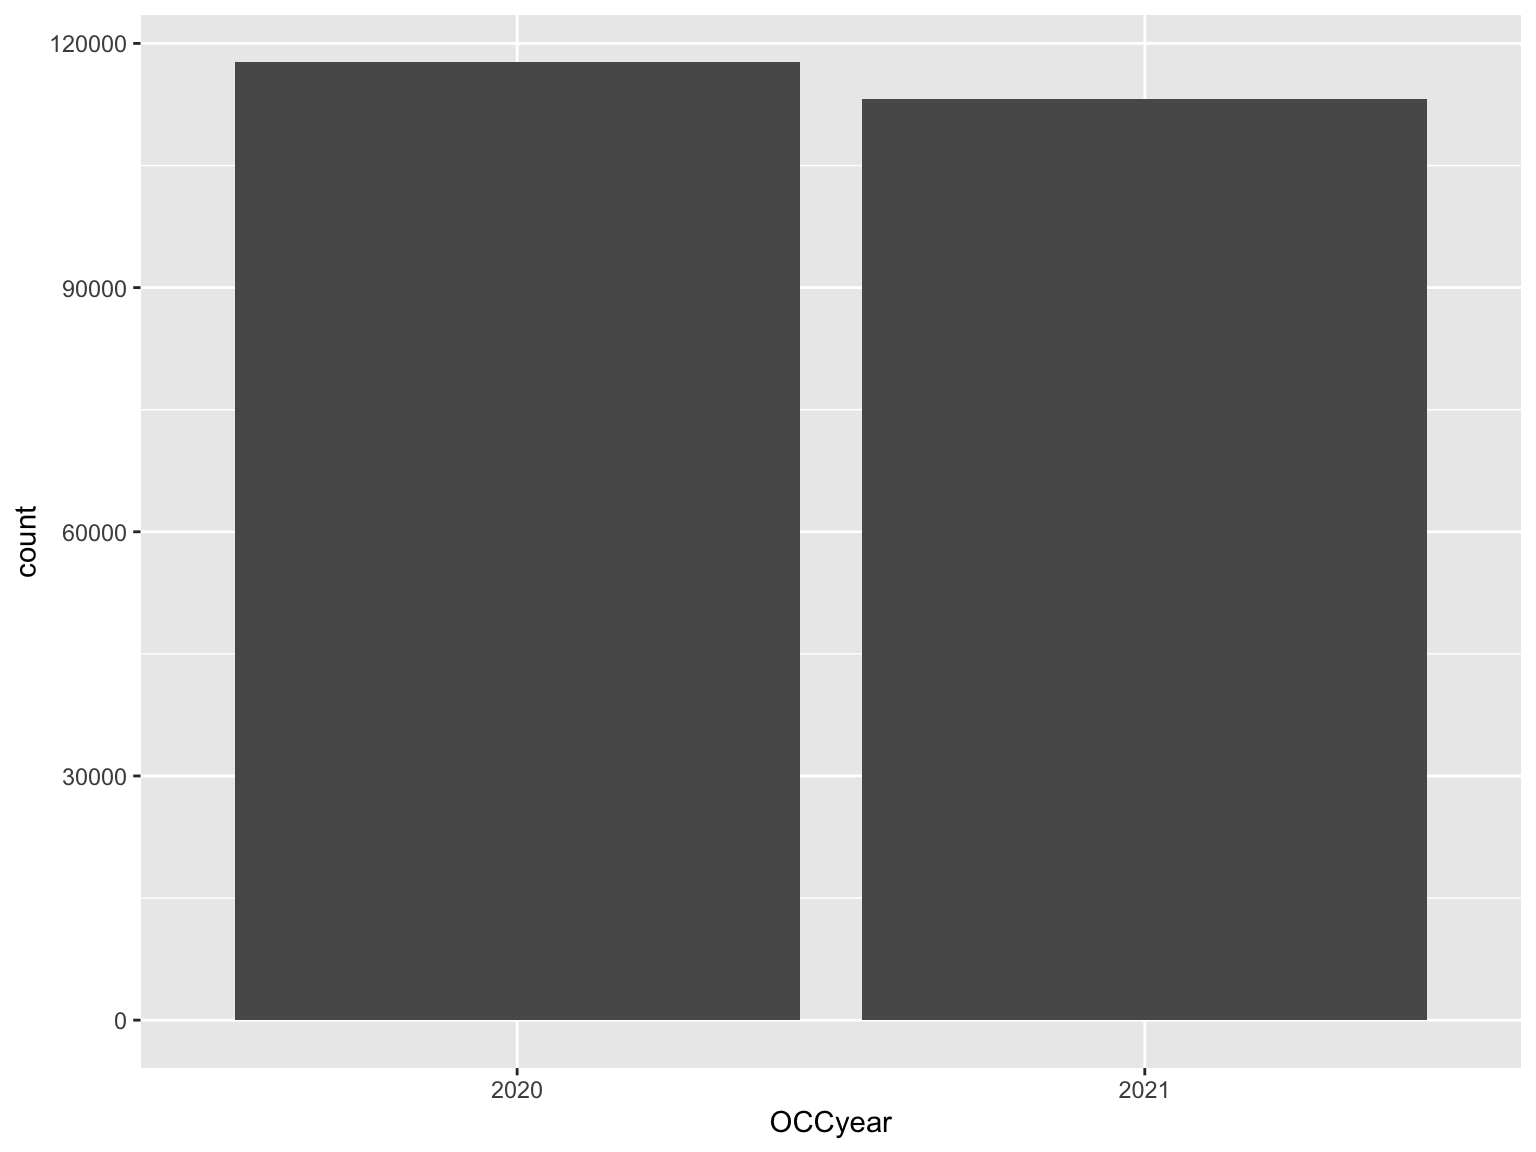
\includegraphics{StatMdlDecisionMaking_files/figure-latex/unnamed-chunk-3-1.pdf}

\begin{Shaded}
\begin{Highlighting}[]
  \CommentTok{\#Assumptions}
    \CommentTok{\#1.Independent observations = Assumed in design of experiment. Durbin{-}Watson could be applied.}
    \CommentTok{\#2.Linearity = Not linear}
      \FunctionTok{par}\NormalTok{(}\AttributeTok{mfrow=}\FunctionTok{c}\NormalTok{(}\DecValTok{2}\NormalTok{,}\DecValTok{2}\NormalTok{))}
      \FunctionTok{plot}\NormalTok{(multiReg) }\CommentTok{\#Residual vs Fitted plot is not linear}
\end{Highlighting}
\end{Shaded}

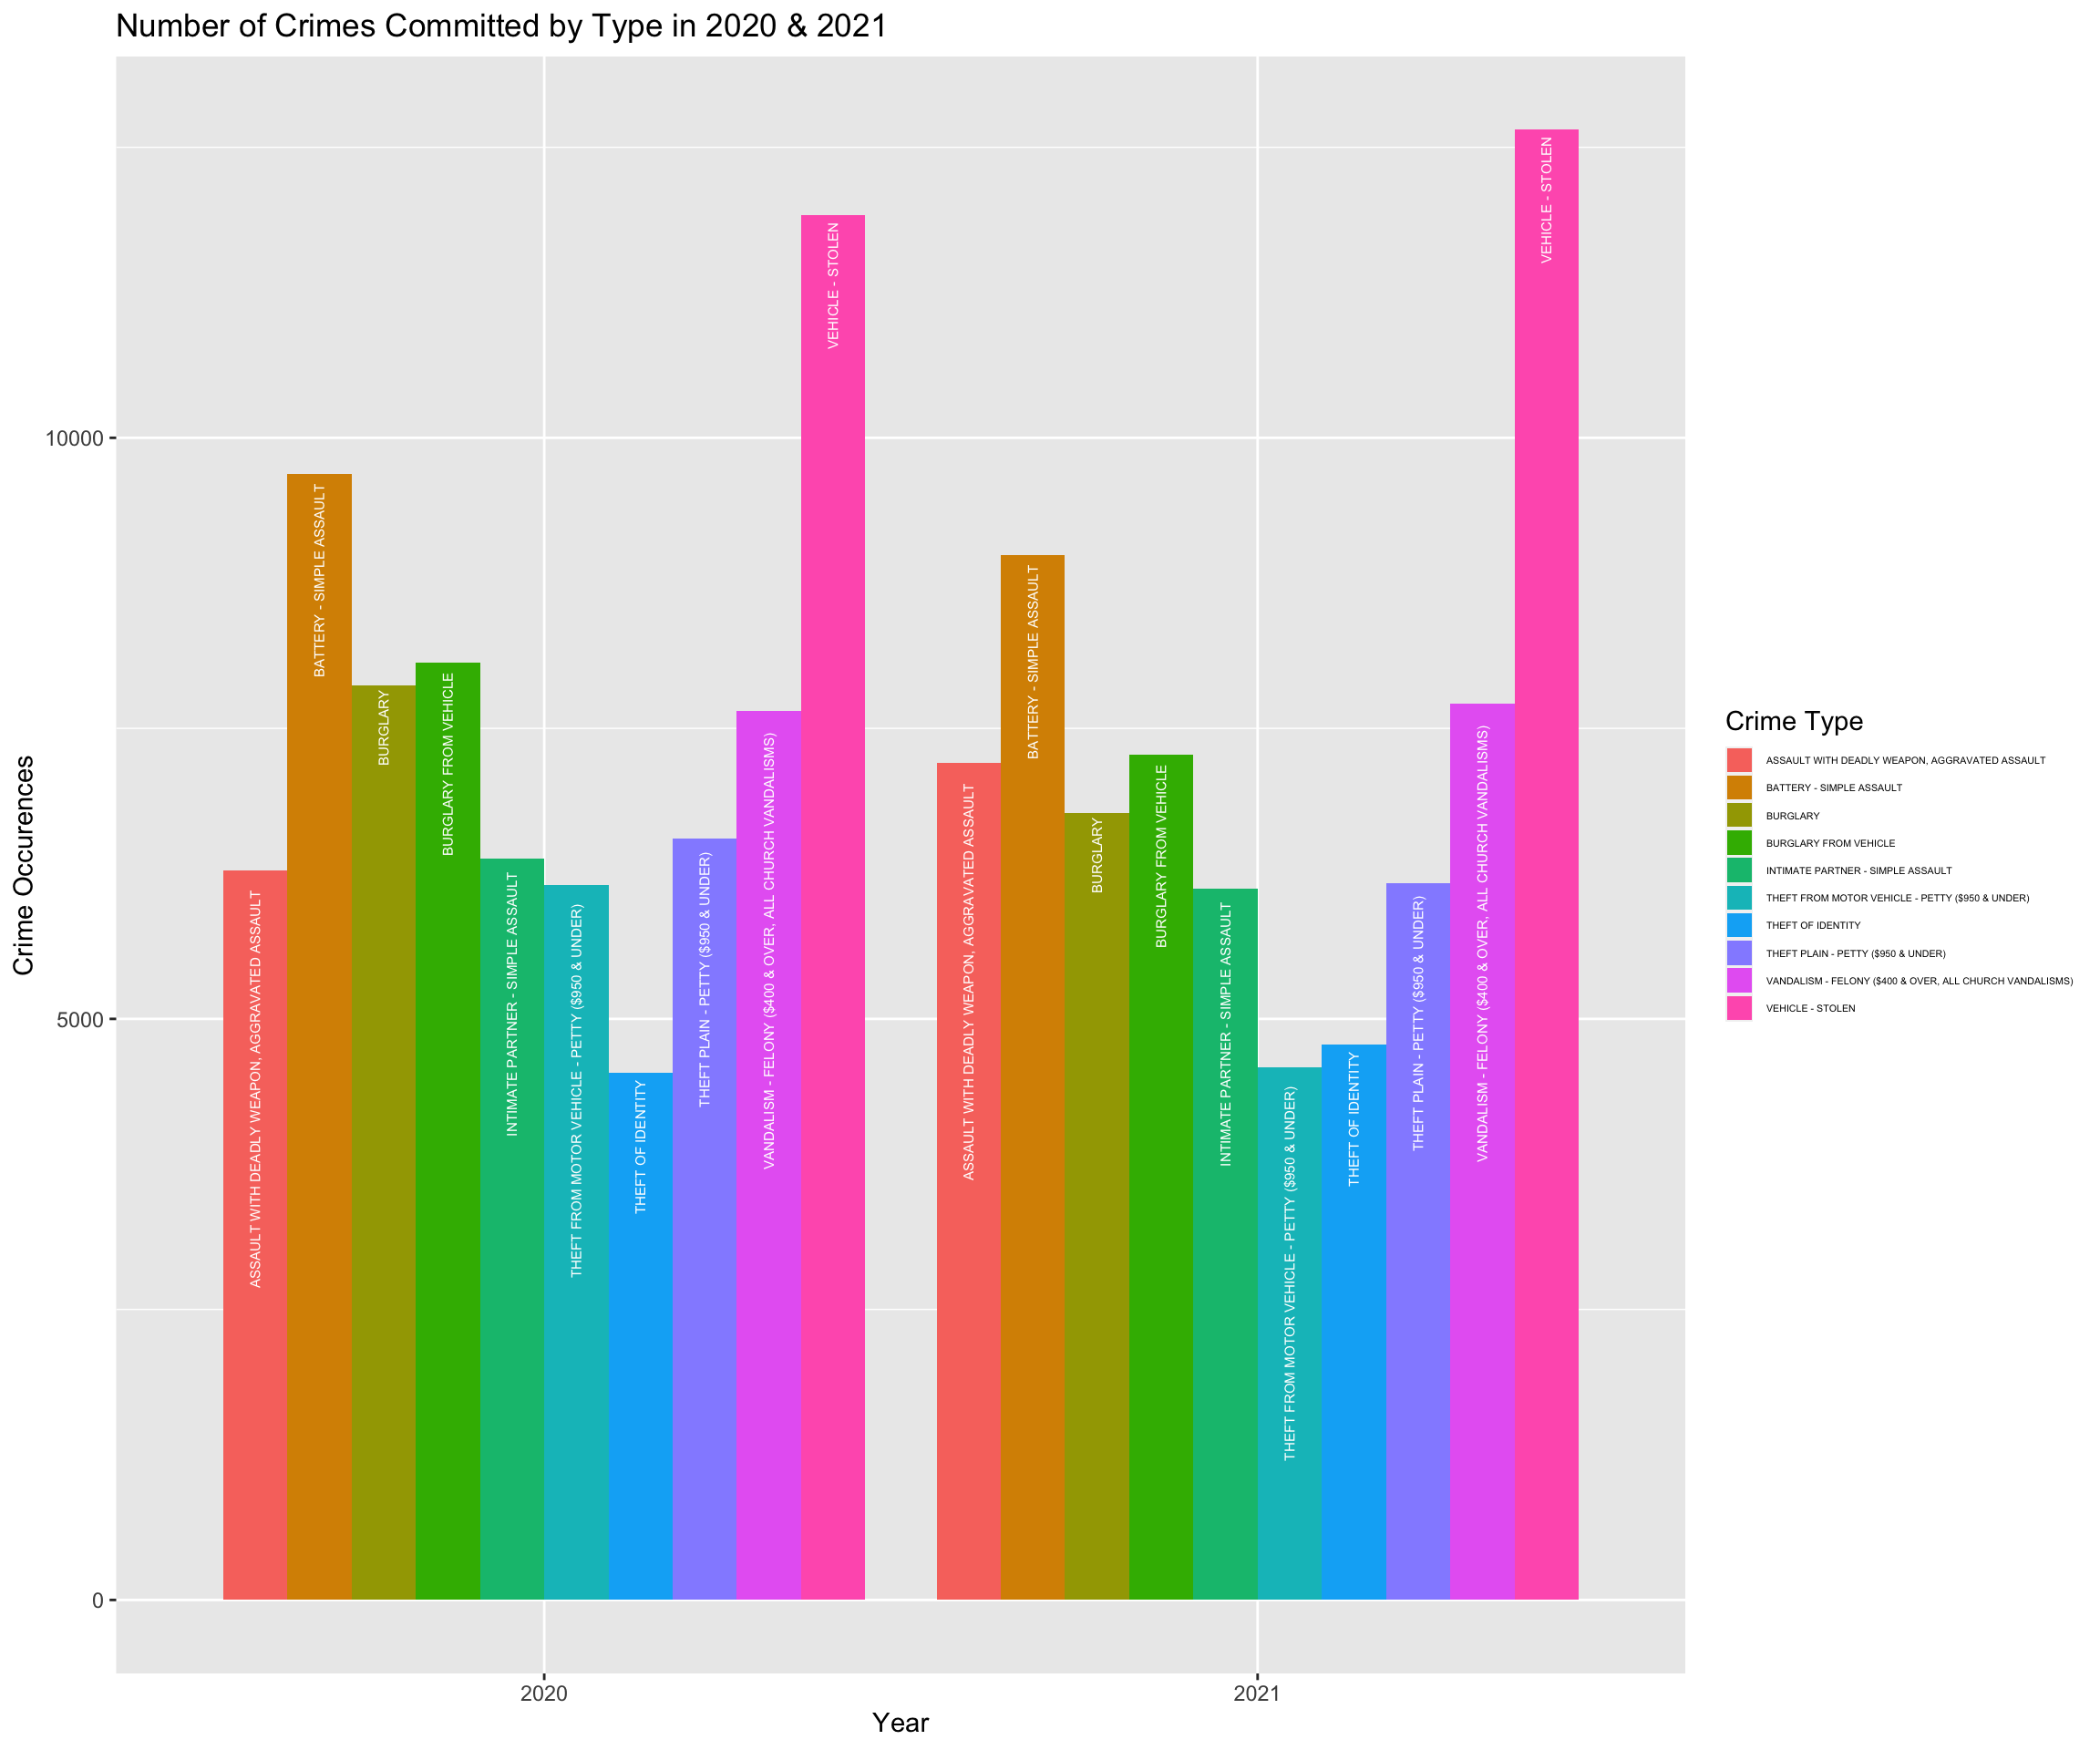
\includegraphics{StatMdlDecisionMaking_files/figure-latex/unnamed-chunk-3-2.pdf}

\begin{Shaded}
\begin{Highlighting}[]
      \FunctionTok{crPlots}\NormalTok{(multiReg) }\CommentTok{\# Most of the variables\textquotesingle{} residuals are not linear}
\end{Highlighting}
\end{Shaded}

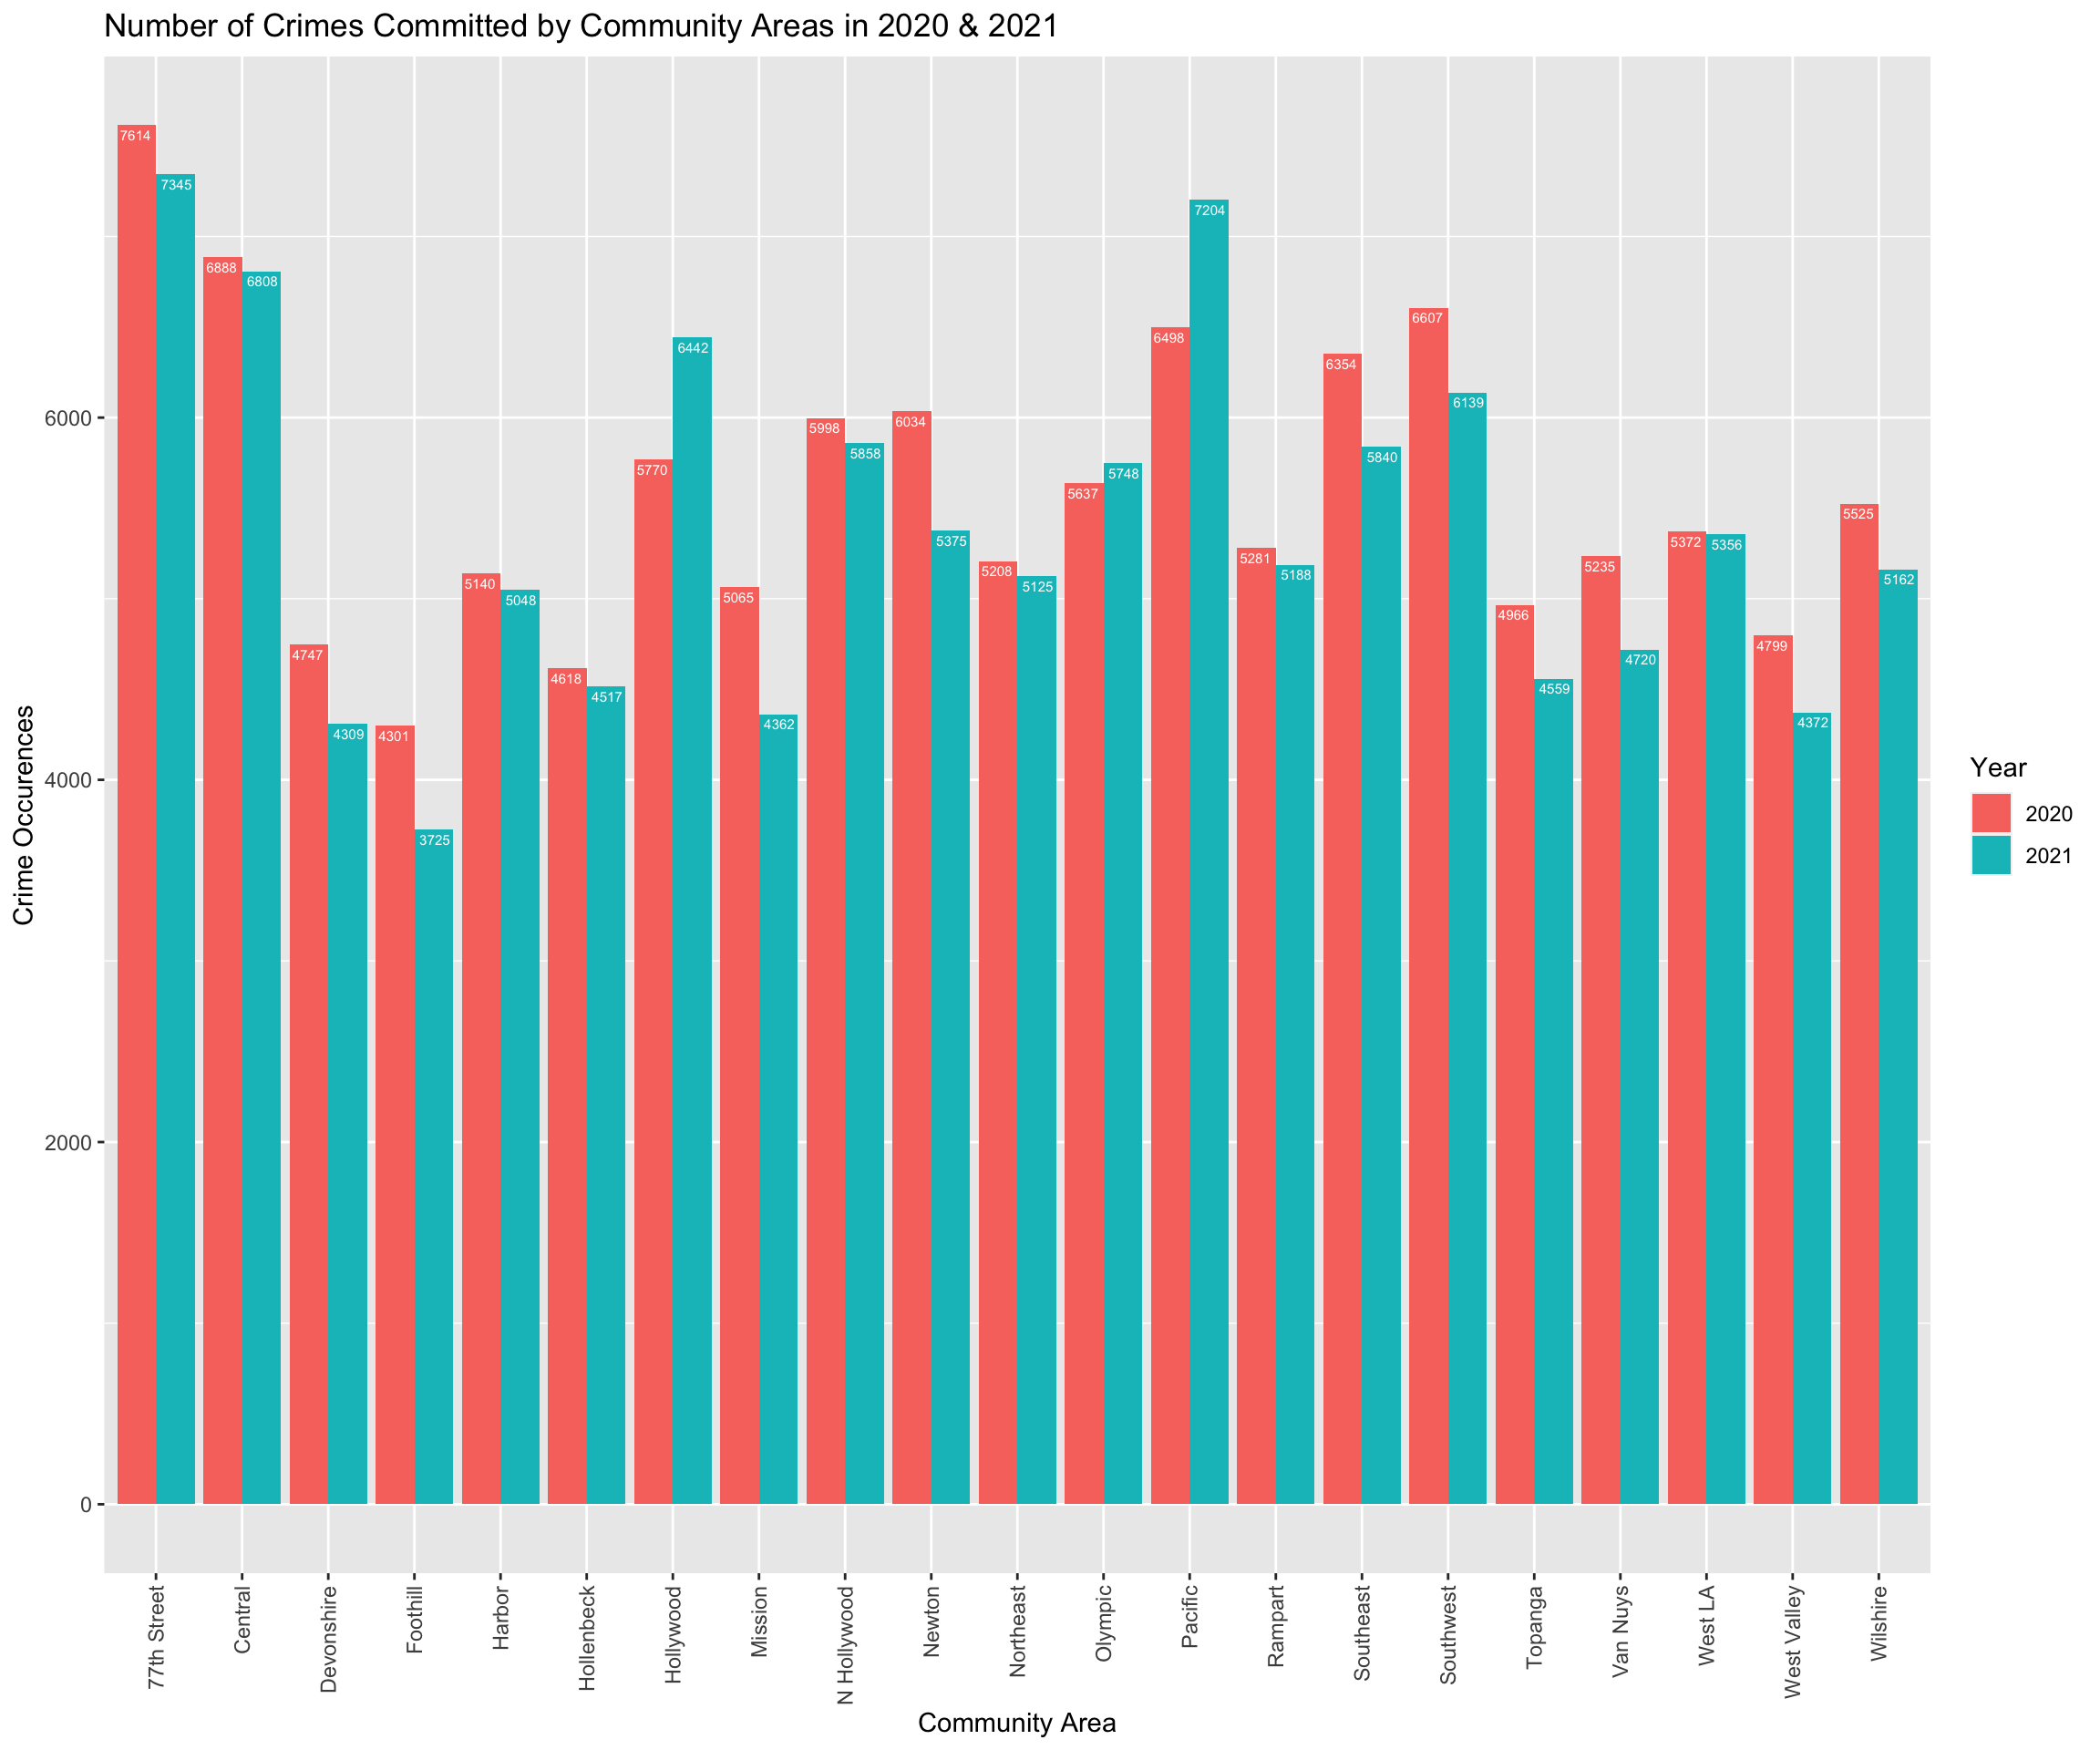
\includegraphics{StatMdlDecisionMaking_files/figure-latex/unnamed-chunk-3-3.pdf}

\begin{Shaded}
\begin{Highlighting}[]
      \CommentTok{\#Maybe transforming lcavol will help. (Even though I see the log transformation has been applied to the relevant variables.)}
\NormalTok{      prostate1 }\OtherTok{\textless{}{-}}\NormalTok{ prostate }\SpecialCharTok{\%\textgreater{}\%} \FunctionTok{mutate}\NormalTok{(}\AttributeTok{lcavol\_c =} \FunctionTok{scale}\NormalTok{(lcavol, }\AttributeTok{scale =} \ConstantTok{FALSE}\NormalTok{))}
\NormalTok{      multiReg1 }\OtherTok{\textless{}{-}} \FunctionTok{lm}\NormalTok{(lpsa }\SpecialCharTok{\textasciitilde{}}\NormalTok{ lcavol\_c}\SpecialCharTok{+} \FunctionTok{I}\NormalTok{(lcavol\_c}\SpecialCharTok{\^{}}\DecValTok{2}\NormalTok{) }\SpecialCharTok{+}\NormalTok{ lweight }\SpecialCharTok{+}\NormalTok{ age }\SpecialCharTok{+}\NormalTok{ lbph }\SpecialCharTok{+}\NormalTok{ svi }\SpecialCharTok{+}\NormalTok{ lcp }\SpecialCharTok{+}\NormalTok{ gleason }\SpecialCharTok{+}\NormalTok{ pgg45, }\AttributeTok{data =}\NormalTok{ prostate1)}
      \FunctionTok{summary}\NormalTok{(multiReg1)}
\end{Highlighting}
\end{Shaded}

\begin{verbatim}
## 
## Call:
## lm(formula = lpsa ~ lcavol_c + I(lcavol_c^2) + lweight + age + 
##     lbph + svi + lcp + gleason + pgg45, data = prostate1)
## 
## Residuals:
##      Min       1Q   Median       3Q      Max 
## -1.73429 -0.37817 -0.01007  0.37917  1.63319 
## 
## Coefficients:
##                Estimate Std. Error t value Pr(>|t|)    
## (Intercept)    1.429977   1.338502   1.068  0.28832    
## lcavol_c       0.594688   0.094361   6.302 1.17e-08 ***
## I(lcavol_c^2)  0.011900   0.051249   0.232  0.81693    
## lweight        0.448784   0.172677   2.599  0.01098 *  
## age           -0.019295   0.011330  -1.703  0.09213 .  
## lbph           0.110603   0.060721   1.821  0.07197 .  
## svi            0.754191   0.250981   3.005  0.00347 ** 
## lcp           -0.109584   0.093203  -1.176  0.24290    
## gleason        0.047276   0.158584   0.298  0.76633    
## pgg45          0.004585   0.004453   1.030  0.30596    
## ---
## Signif. codes:  0 '***' 0.001 '**' 0.01 '*' 0.05 '.' 0.1 ' ' 1
## 
## Residual standard error: 0.7123 on 87 degrees of freedom
## Multiple R-squared:  0.655,  Adjusted R-squared:  0.6193 
## F-statistic: 18.35 on 9 and 87 DF,  p-value: < 2.2e-16
\end{verbatim}

\begin{Shaded}
\begin{Highlighting}[]
      \FunctionTok{crPlots}\NormalTok{(multiReg1)}\CommentTok{\#It barely changed, so I will not be using this transformation going forward, but I wanted to check.}
\end{Highlighting}
\end{Shaded}

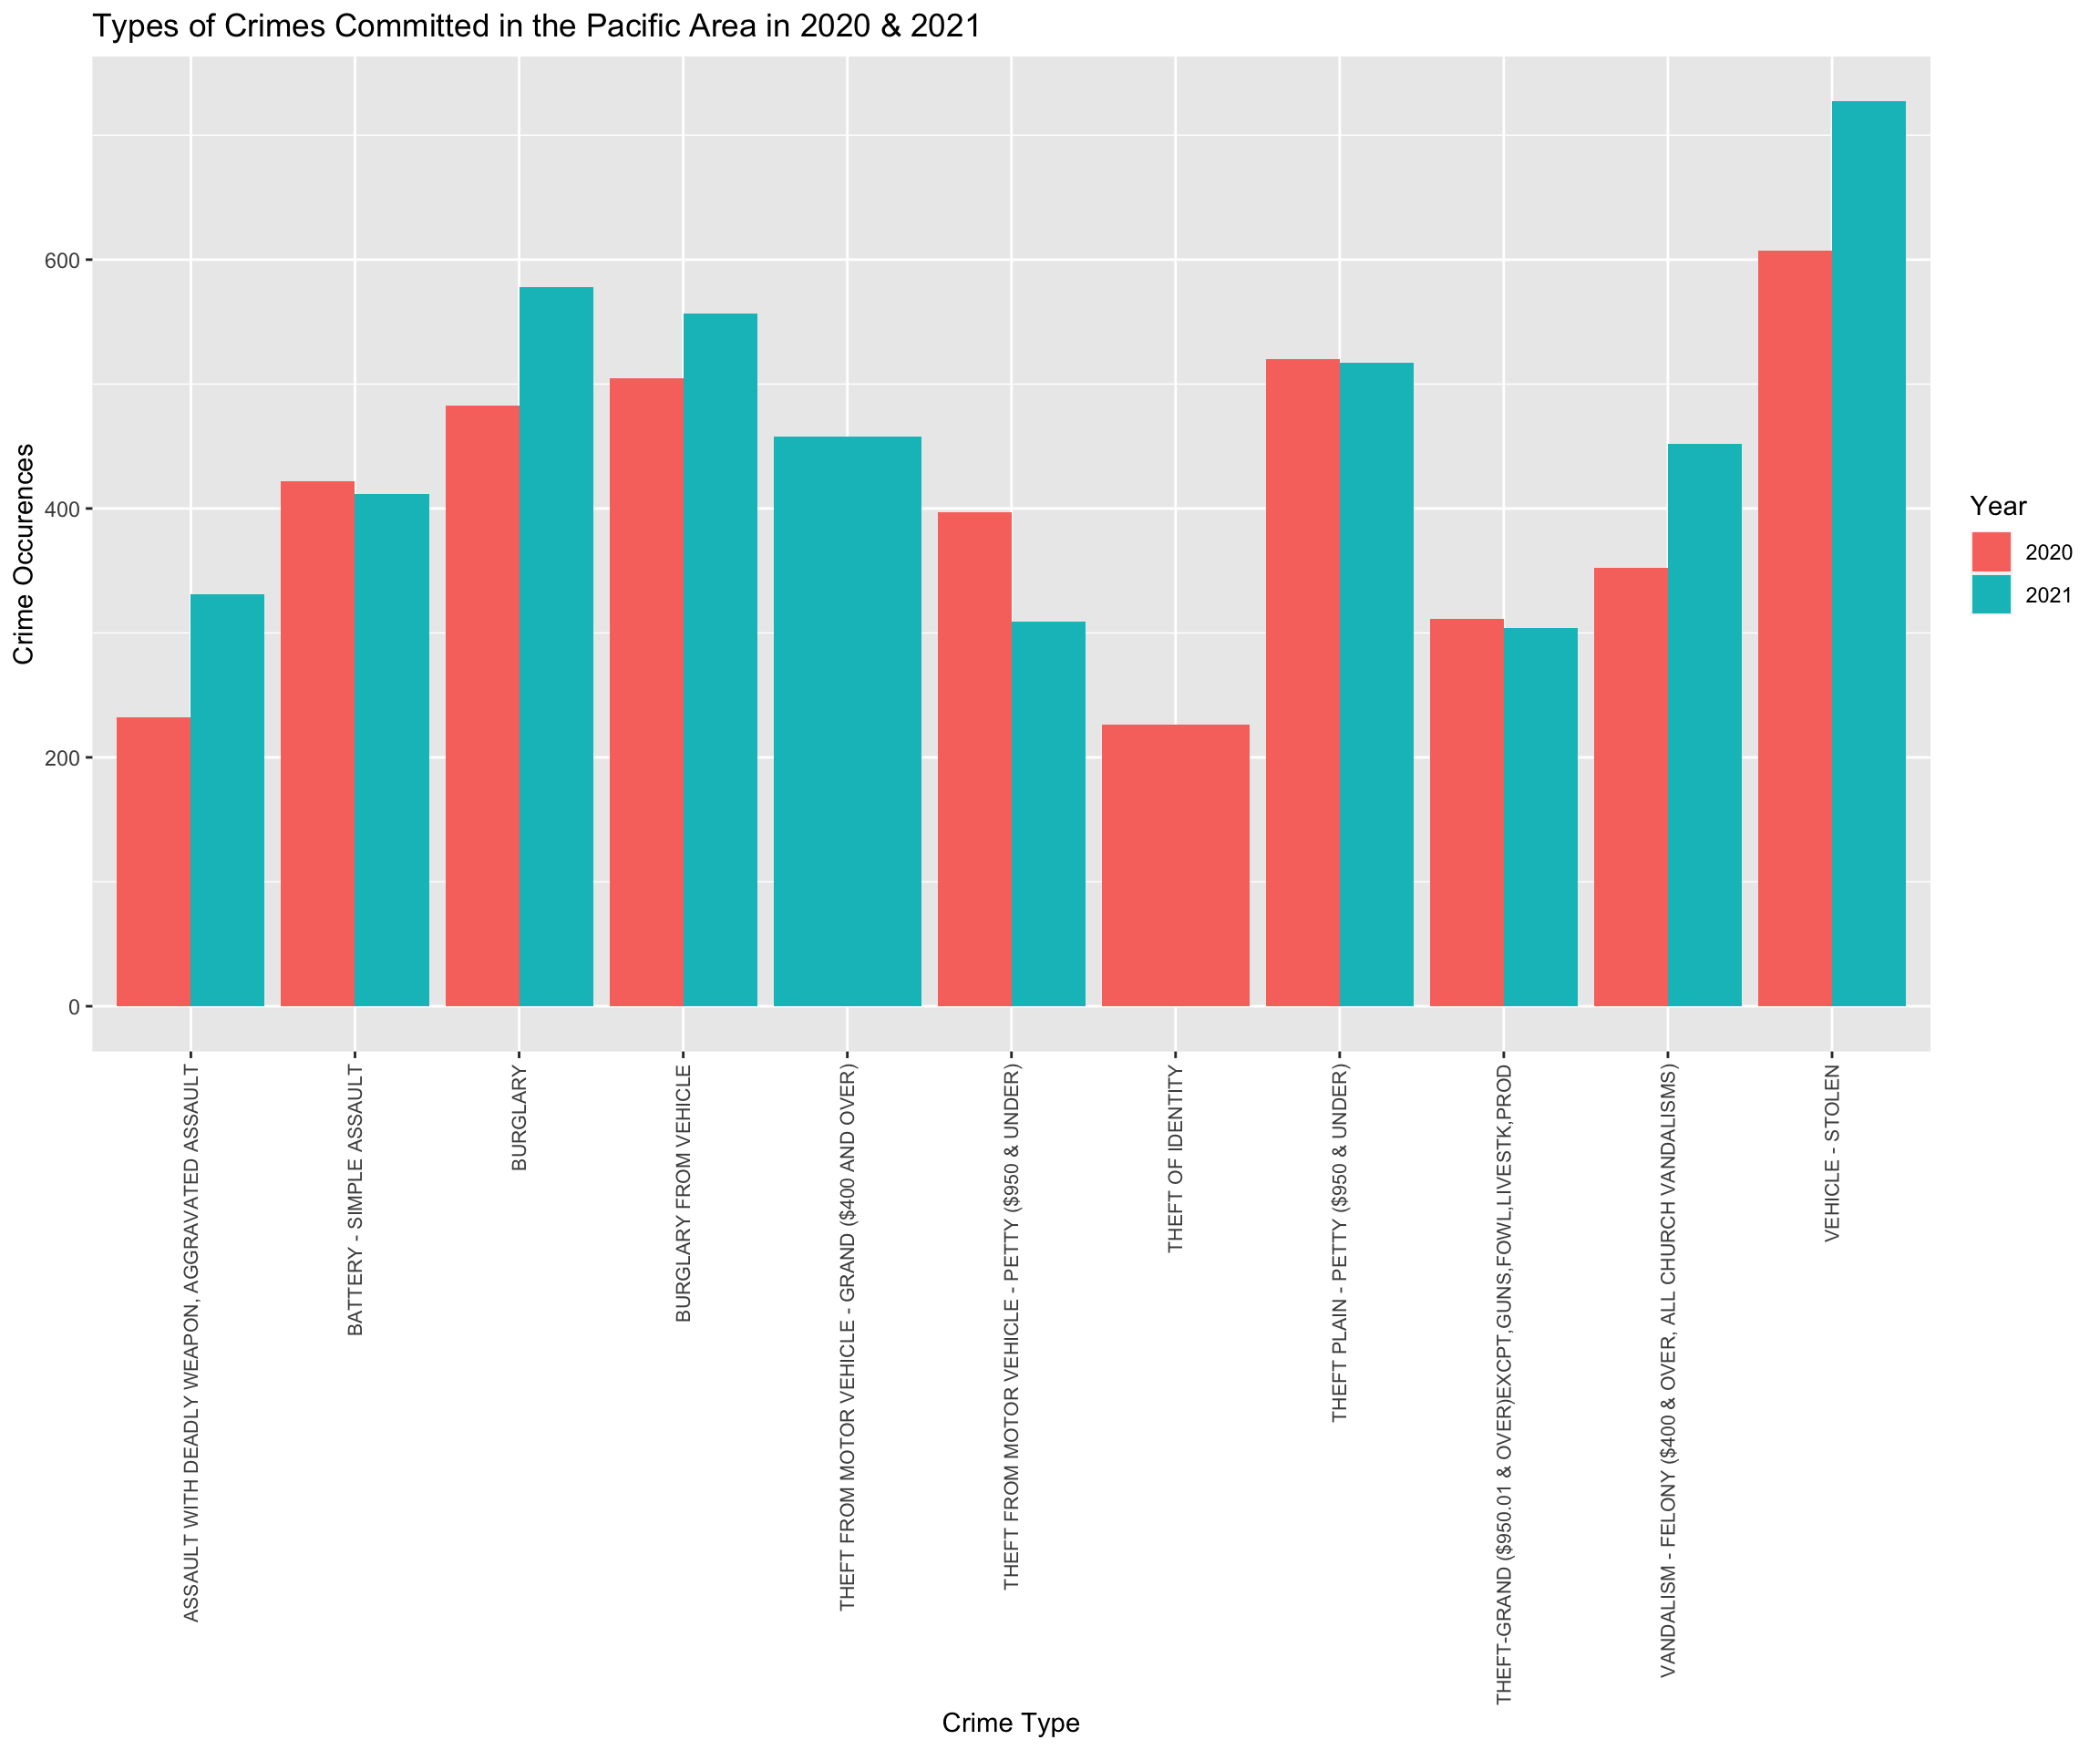
\includegraphics{StatMdlDecisionMaking_files/figure-latex/unnamed-chunk-3-4.pdf}

\begin{Shaded}
\begin{Highlighting}[]
    \CommentTok{\#3 Homoscedasticity/ constant variability = Not homoscedastic.}
      \FunctionTok{par}\NormalTok{(}\AttributeTok{mfrow=}\FunctionTok{c}\NormalTok{(}\DecValTok{2}\NormalTok{,}\DecValTok{2}\NormalTok{))}
      \FunctionTok{plot}\NormalTok{(multiReg)}\CommentTok{\#See plot(multiReg)\textquotesingle{}s Scale{-}Location plot. The line is not horizontal enough to be homoscedastic. Since a log transformation has already been performed it won\textquotesingle{}t get much straighter than this.}
\end{Highlighting}
\end{Shaded}

\includegraphics{StatMdlDecisionMaking_files/figure-latex/unnamed-chunk-3-5.pdf}

\begin{Shaded}
\begin{Highlighting}[]
    \CommentTok{\#4 Normality of Residuals = Residuals are not the most normal. It could be worse, but it is not great.}
      \CommentTok{\#See plot(multiReg)\textquotesingle{}s Nornal Q{-}Q plot OR the following: }
\NormalTok{      pros.data }\OtherTok{\textless{}{-}} \FunctionTok{augment}\NormalTok{(multiReg)}\CommentTok{\# get the residuals}
      \FunctionTok{ggplot}\NormalTok{(pros.data, }\FunctionTok{aes}\NormalTok{(}\AttributeTok{sample =}\NormalTok{ .resid)) }\SpecialCharTok{+}
\FunctionTok{geom\_qq}\NormalTok{() }\SpecialCharTok{+}
\FunctionTok{stat\_qq\_line}\NormalTok{(}\AttributeTok{color =} \StringTok{"green"}\NormalTok{) }\CommentTok{\#Doesn\textquotesingle{}t follow a straight line, not normal, but close}
\end{Highlighting}
\end{Shaded}

\includegraphics{StatMdlDecisionMaking_files/figure-latex/unnamed-chunk-3-6.pdf}

\begin{Shaded}
\begin{Highlighting}[]
     \FunctionTok{ggplot}\NormalTok{(pros.data, }\FunctionTok{aes}\NormalTok{(}\AttributeTok{x =}\NormalTok{ .resid)) }\SpecialCharTok{+}
\FunctionTok{geom\_histogram}\NormalTok{(}\AttributeTok{bins =} \DecValTok{35}\NormalTok{) }\CommentTok{\#Normal enough, maybe a little platykurtic}
\end{Highlighting}
\end{Shaded}

\includegraphics{StatMdlDecisionMaking_files/figure-latex/unnamed-chunk-3-7.pdf}

\begin{Shaded}
\begin{Highlighting}[]
\NormalTok{     (}\FunctionTok{length}\NormalTok{(}\FunctionTok{boxplot}\NormalTok{(prostate}\SpecialCharTok{$}\NormalTok{lpsa, }\AttributeTok{plot=}\NormalTok{F)}\SpecialCharTok{$}\NormalTok{out)}\SpecialCharTok{/}\DecValTok{97}\NormalTok{)}\SpecialCharTok{*}\DecValTok{100} \CommentTok{\#I could remove outliers here, but I\textquotesingle{}ve decided against it since there are so many of them (4.1\% of data are outliers). That is too much to cut out}
\end{Highlighting}
\end{Shaded}

\begin{verbatim}
## [1] 4.123711
\end{verbatim}

\begin{Shaded}
\begin{Highlighting}[]
    \CommentTok{\#5 No multicollinearity = Multicollinearity is present in a number of variables.}
      \FunctionTok{ggpairs}\NormalTok{(}\AttributeTok{data=}\NormalTok{prostate)}
\end{Highlighting}
\end{Shaded}

\includegraphics{StatMdlDecisionMaking_files/figure-latex/unnamed-chunk-3-8.pdf}

\begin{Shaded}
\begin{Highlighting}[]
      \FunctionTok{ggcorr}\NormalTok{(prostate)}\CommentTok{\#gleason \& pgg45 are highly correlated and that makes sense. Pgg45 is based on gleason scores. lpsa \& lcavol, lcp\&svi, lcp\&lcavol, lcp\&pgg45,  lpsa\&svi, and lcp\&gleason are all relatively correlated, so multicollinearity is present.}
\end{Highlighting}
\end{Shaded}

\includegraphics{StatMdlDecisionMaking_files/figure-latex/unnamed-chunk-3-9.pdf}

\begin{Shaded}
\begin{Highlighting}[]
\CommentTok{\#Which model best fits}
  \CommentTok{\#by significance = lcavol, lweight, svi, with age and bph\textquotesingle{}s p{-}val= 0.1}
  \CommentTok{\#by backward BIC = lcavol, lweight, svi}
\NormalTok{    multiReg\_back }\OtherTok{\textless{}{-}} \FunctionTok{lm}\NormalTok{(lpsa }\SpecialCharTok{\textasciitilde{}}\NormalTok{ .,prostate)}
\NormalTok{    n }\OtherTok{\textless{}{-}} \FunctionTok{nrow}\NormalTok{(prostate)}
\NormalTok{    back.bic }\OtherTok{\textless{}{-}} \FunctionTok{step}\NormalTok{(multiReg\_back, }\AttributeTok{direction =} \StringTok{"backward"}\NormalTok{,  }\AttributeTok{k=} \FunctionTok{log}\NormalTok{(n), }\AttributeTok{trace =} \DecValTok{0}\NormalTok{)}
\NormalTok{    back.bic}
\end{Highlighting}
\end{Shaded}

\begin{verbatim}
## 
## Call:
## lm(formula = lpsa ~ lcavol + lweight + svi, data = prostate)
## 
## Coefficients:
## (Intercept)       lcavol      lweight          svi  
##     -0.2681       0.5516       0.5085       0.6662
\end{verbatim}

\begin{Shaded}
\begin{Highlighting}[]
  \CommentTok{\#by backward AIC = lcavol, lweight, svi, age, lbph,}
\NormalTok{    multiReg\_back }\OtherTok{\textless{}{-}} \FunctionTok{lm}\NormalTok{(lpsa }\SpecialCharTok{\textasciitilde{}}\NormalTok{ .,prostate)}
\NormalTok{    back.aic }\OtherTok{\textless{}{-}} \FunctionTok{step}\NormalTok{(multiReg\_back, }\AttributeTok{direction =} \StringTok{"backward"}\NormalTok{, }\AttributeTok{trace =} \DecValTok{0}\NormalTok{)}
\NormalTok{    back.aic}
\end{Highlighting}
\end{Shaded}

\begin{verbatim}
## 
## Call:
## lm(formula = lpsa ~ lcavol + lweight + age + lbph + svi, data = prostate)
## 
## Coefficients:
## (Intercept)       lcavol      lweight          age         lbph          svi  
##     0.95100      0.56561      0.42369     -0.01489      0.11184      0.72095
\end{verbatim}

\begin{Shaded}
\begin{Highlighting}[]
\CommentTok{\#Best model showdown!}
\NormalTok{multiReg\_best1 }\OtherTok{\textless{}{-}} \FunctionTok{lm}\NormalTok{(lpsa }\SpecialCharTok{\textasciitilde{}}\NormalTok{ lcavol }\SpecialCharTok{+}\NormalTok{ lweight }\SpecialCharTok{+}\NormalTok{ svi }\SpecialCharTok{+}\NormalTok{ age }\SpecialCharTok{+}\NormalTok{ lbph, prostate)}
\FunctionTok{summary}\NormalTok{(multiReg\_best1)}\CommentTok{\#Adjusted r\^{}2 = 0.6245, \#The winner}
\end{Highlighting}
\end{Shaded}

\begin{verbatim}
## 
## Call:
## lm(formula = lpsa ~ lcavol + lweight + svi + age + lbph, data = prostate)
## 
## Residuals:
##      Min       1Q   Median       3Q      Max 
## -1.83505 -0.39396  0.00414  0.46336  1.57888 
## 
## Coefficients:
##             Estimate Std. Error t value Pr(>|t|)    
## (Intercept)  0.95100    0.83175   1.143 0.255882    
## lcavol       0.56561    0.07459   7.583 2.77e-11 ***
## lweight      0.42369    0.16687   2.539 0.012814 *  
## svi          0.72095    0.20902   3.449 0.000854 ***
## age         -0.01489    0.01075  -1.385 0.169528    
## lbph         0.11184    0.05805   1.927 0.057160 .  
## ---
## Signif. codes:  0 '***' 0.001 '**' 0.01 '*' 0.05 '.' 0.1 ' ' 1
## 
## Residual standard error: 0.7073 on 91 degrees of freedom
## Multiple R-squared:  0.6441, Adjusted R-squared:  0.6245 
## F-statistic: 32.94 on 5 and 91 DF,  p-value: < 2.2e-16
\end{verbatim}

\begin{Shaded}
\begin{Highlighting}[]
\NormalTok{multiReg\_best2 }\OtherTok{\textless{}{-}} \FunctionTok{lm}\NormalTok{(lpsa }\SpecialCharTok{\textasciitilde{}}\NormalTok{ lcavol }\SpecialCharTok{+}\NormalTok{ lweight }\SpecialCharTok{+}\NormalTok{ svi, prostate)}
\FunctionTok{summary}\NormalTok{(multiReg\_best2)}\CommentTok{\#Adjusted r\^{}2 = 0.6144}
\end{Highlighting}
\end{Shaded}

\begin{verbatim}
## 
## Call:
## lm(formula = lpsa ~ lcavol + lweight + svi, data = prostate)
## 
## Residuals:
##      Min       1Q   Median       3Q      Max 
## -1.72964 -0.45764  0.02812  0.46403  1.57013 
## 
## Coefficients:
##             Estimate Std. Error t value Pr(>|t|)    
## (Intercept) -0.26809    0.54350  -0.493  0.62298    
## lcavol       0.55164    0.07467   7.388  6.3e-11 ***
## lweight      0.50854    0.15017   3.386  0.00104 ** 
## svi          0.66616    0.20978   3.176  0.00203 ** 
## ---
## Signif. codes:  0 '***' 0.001 '**' 0.01 '*' 0.05 '.' 0.1 ' ' 1
## 
## Residual standard error: 0.7168 on 93 degrees of freedom
## Multiple R-squared:  0.6264, Adjusted R-squared:  0.6144 
## F-statistic: 51.99 on 3 and 93 DF,  p-value: < 2.2e-16
\end{verbatim}

\begin{Shaded}
\begin{Highlighting}[]
\CommentTok{\#The R\^{}2 for the first one is higher and therefore the predictor variables explain more of the variance with multiReg\_best1 than multiReg\_best2. Also the researchers are looking for more a predictive model than an explanatory model, so keeping age and lbph is the better choice. }
\end{Highlighting}
\end{Shaded}

Question 4: 1.Noted 2.Regression with Interaction term Null Hypothesis:
There is no effect of region on infant mortality rates even with the
influence of income per capita accounted for. Alternative Hypothesis:
There is an effect of region on infant mortality rates even with the
influence of income per capita accounted for. Significance will be set
to 0.10.

Results: P-value: 4.55e-13 There is affect of region on infant mortality
rates even with the influence of income per capita accounted for. The
Reject the Null. Adjusted R-squared = 0.227, the model explains 22.7\%
of the variability seen Coefficients are significant = Africa, Americas,
and Europe regions along with interaction between Americas region and
income Residual standard error=79.83 F-stat= 5.194

Conclusion: There is an effect of region on infant mortality rate. With
the comparison point being Africa, the Americas and Europe decrease in
mortality as compared to Africa. The Americas this especially true when
factoring in the association income, which decreases as compared to
Africa.

Comparing the two models, we find

\begin{Shaded}
\begin{Highlighting}[]
\CommentTok{\#1}
\CommentTok{\#Run Regression for Assumption functions to makes sense}
\NormalTok{Reg }\OtherTok{\textless{}{-}} \FunctionTok{lm}\NormalTok{(mortality }\SpecialCharTok{\textasciitilde{}}\NormalTok{ region, }\AttributeTok{data =}\NormalTok{ infmort)}
\FunctionTok{summary}\NormalTok{(Reg)}
\end{Highlighting}
\end{Shaded}

\begin{verbatim}
## 
## Call:
## lm(formula = mortality ~ region, data = infmort)
## 
## Residuals:
##    Min     1Q Median     3Q    Max 
## -87.29 -37.52  -5.76  16.91 553.83 
## 
## Coefficients:
##                Estimate Std. Error t value Pr(>|t|)    
## (Intercept)      142.29      13.64  10.431  < 2e-16 ***
## regionAmericas   -87.17      21.76  -4.005 0.000122 ***
## regionAsia       -46.12      20.50  -2.249 0.026755 *  
## regionEurope    -123.04      23.19  -5.306 7.07e-07 ***
## ---
## Signif. codes:  0 '***' 0.001 '**' 0.01 '*' 0.05 '.' 0.1 ' ' 1
## 
## Residual standard error: 79.54 on 97 degrees of freedom
##   (4 observations deleted due to missingness)
## Multiple R-squared:  0.2556, Adjusted R-squared:  0.2326 
## F-statistic:  11.1 on 3 and 97 DF,  p-value: 2.494e-06
\end{verbatim}

\begin{Shaded}
\begin{Highlighting}[]
\CommentTok{\#EDA}
  \CommentTok{\#Preliminary EDA}
  \FunctionTok{dim}\NormalTok{(infmort)}
\end{Highlighting}
\end{Shaded}

\begin{verbatim}
## [1] 105   4
\end{verbatim}

\begin{Shaded}
\begin{Highlighting}[]
  \FunctionTok{str}\NormalTok{(infmort)}
\end{Highlighting}
\end{Shaded}

\begin{verbatim}
## 'data.frame':    105 obs. of  4 variables:
##  $ region   : chr  "Asia" "Europe" "Europe" "Americas" ...
##  $ income   : int  3426 3350 3346 4751 5029 3312 3403 5040 2009 2298 ...
##  $ mortality: num  26.7 23.7 17 16.8 13.5 10.1 12.9 20.4 17.8 25.7 ...
##  $ oil      : chr  "no oil exports" "no oil exports" "no oil exports" "no oil exports" ...
\end{verbatim}

\begin{Shaded}
\begin{Highlighting}[]
  \FunctionTok{sum}\NormalTok{(}\FunctionTok{is.na}\NormalTok{(infmort))}\CommentTok{\#4 NAs in mortality}
\end{Highlighting}
\end{Shaded}

\begin{verbatim}
## [1] 4
\end{verbatim}

\begin{Shaded}
\begin{Highlighting}[]
\NormalTok{  infmort }\OtherTok{\textless{}{-}} \FunctionTok{na.omit}\NormalTok{(infmort) }
  \FunctionTok{summary}\NormalTok{(infmort)}
\end{Highlighting}
\end{Shaded}

\begin{verbatim}
##     region              income       mortality          oil           
##  Length:101         Min.   :  50   Min.   :  9.60   Length:101        
##  Class :character   1st Qu.: 130   1st Qu.: 26.20   Class :character  
##  Mode  :character   Median : 334   Median : 60.60   Mode  :character  
##                     Mean   :1022   Mean   : 89.05                     
##                     3rd Qu.:1191   3rd Qu.:129.40                     
##                     Max.   :5596   Max.   :650.00
\end{verbatim}

\begin{Shaded}
\begin{Highlighting}[]
\NormalTok{  infmort }\SpecialCharTok{\%\textgreater{}\%}
\FunctionTok{group\_by}\NormalTok{(region) }\SpecialCharTok{\%\textgreater{}\%}
\FunctionTok{summarise}\NormalTok{(}\AttributeTok{mean =} \FunctionTok{mean}\NormalTok{(mortality)) }\SpecialCharTok{\%\textgreater{}\%}\NormalTok{ pander}
\end{Highlighting}
\end{Shaded}

\begin{longtable}[]{@{}
  >{\centering\arraybackslash}p{(\columnwidth - 2\tabcolsep) * \real{0.1528}}
  >{\centering\arraybackslash}p{(\columnwidth - 2\tabcolsep) * \real{0.1111}}@{}}
\toprule\noalign{}
\begin{minipage}[b]{\linewidth}\centering
region
\end{minipage} & \begin{minipage}[b]{\linewidth}\centering
mean
\end{minipage} \\
\midrule\noalign{}
\endhead
\bottomrule\noalign{}
\endlastfoot
Africa & 142.3 \\
Americas & 55.12 \\
Asia & 96.17 \\
Europe & 19.26 \\
\end{longtable}

\begin{Shaded}
\begin{Highlighting}[]
  \FunctionTok{levels}\NormalTok{(}\FunctionTok{factor}\NormalTok{(infmort}\SpecialCharTok{$}\NormalTok{region))}
\end{Highlighting}
\end{Shaded}

\begin{verbatim}
## [1] "Africa"   "Americas" "Asia"     "Europe"
\end{verbatim}

\begin{Shaded}
\begin{Highlighting}[]
  \CommentTok{\#Plots}
  \FunctionTok{ggplot}\NormalTok{(infmort, }\FunctionTok{aes}\NormalTok{(mortality, }\AttributeTok{fill=}\NormalTok{ region))}\SpecialCharTok{+}
        \FunctionTok{geom\_boxplot}\NormalTok{()}\SpecialCharTok{+}
      \FunctionTok{facet\_grid}\NormalTok{(region }\SpecialCharTok{\textasciitilde{}}\NormalTok{ .)}\SpecialCharTok{+}
    \FunctionTok{theme}\NormalTok{(}\AttributeTok{legend.position =} \StringTok{"none"}\NormalTok{)}
\end{Highlighting}
\end{Shaded}

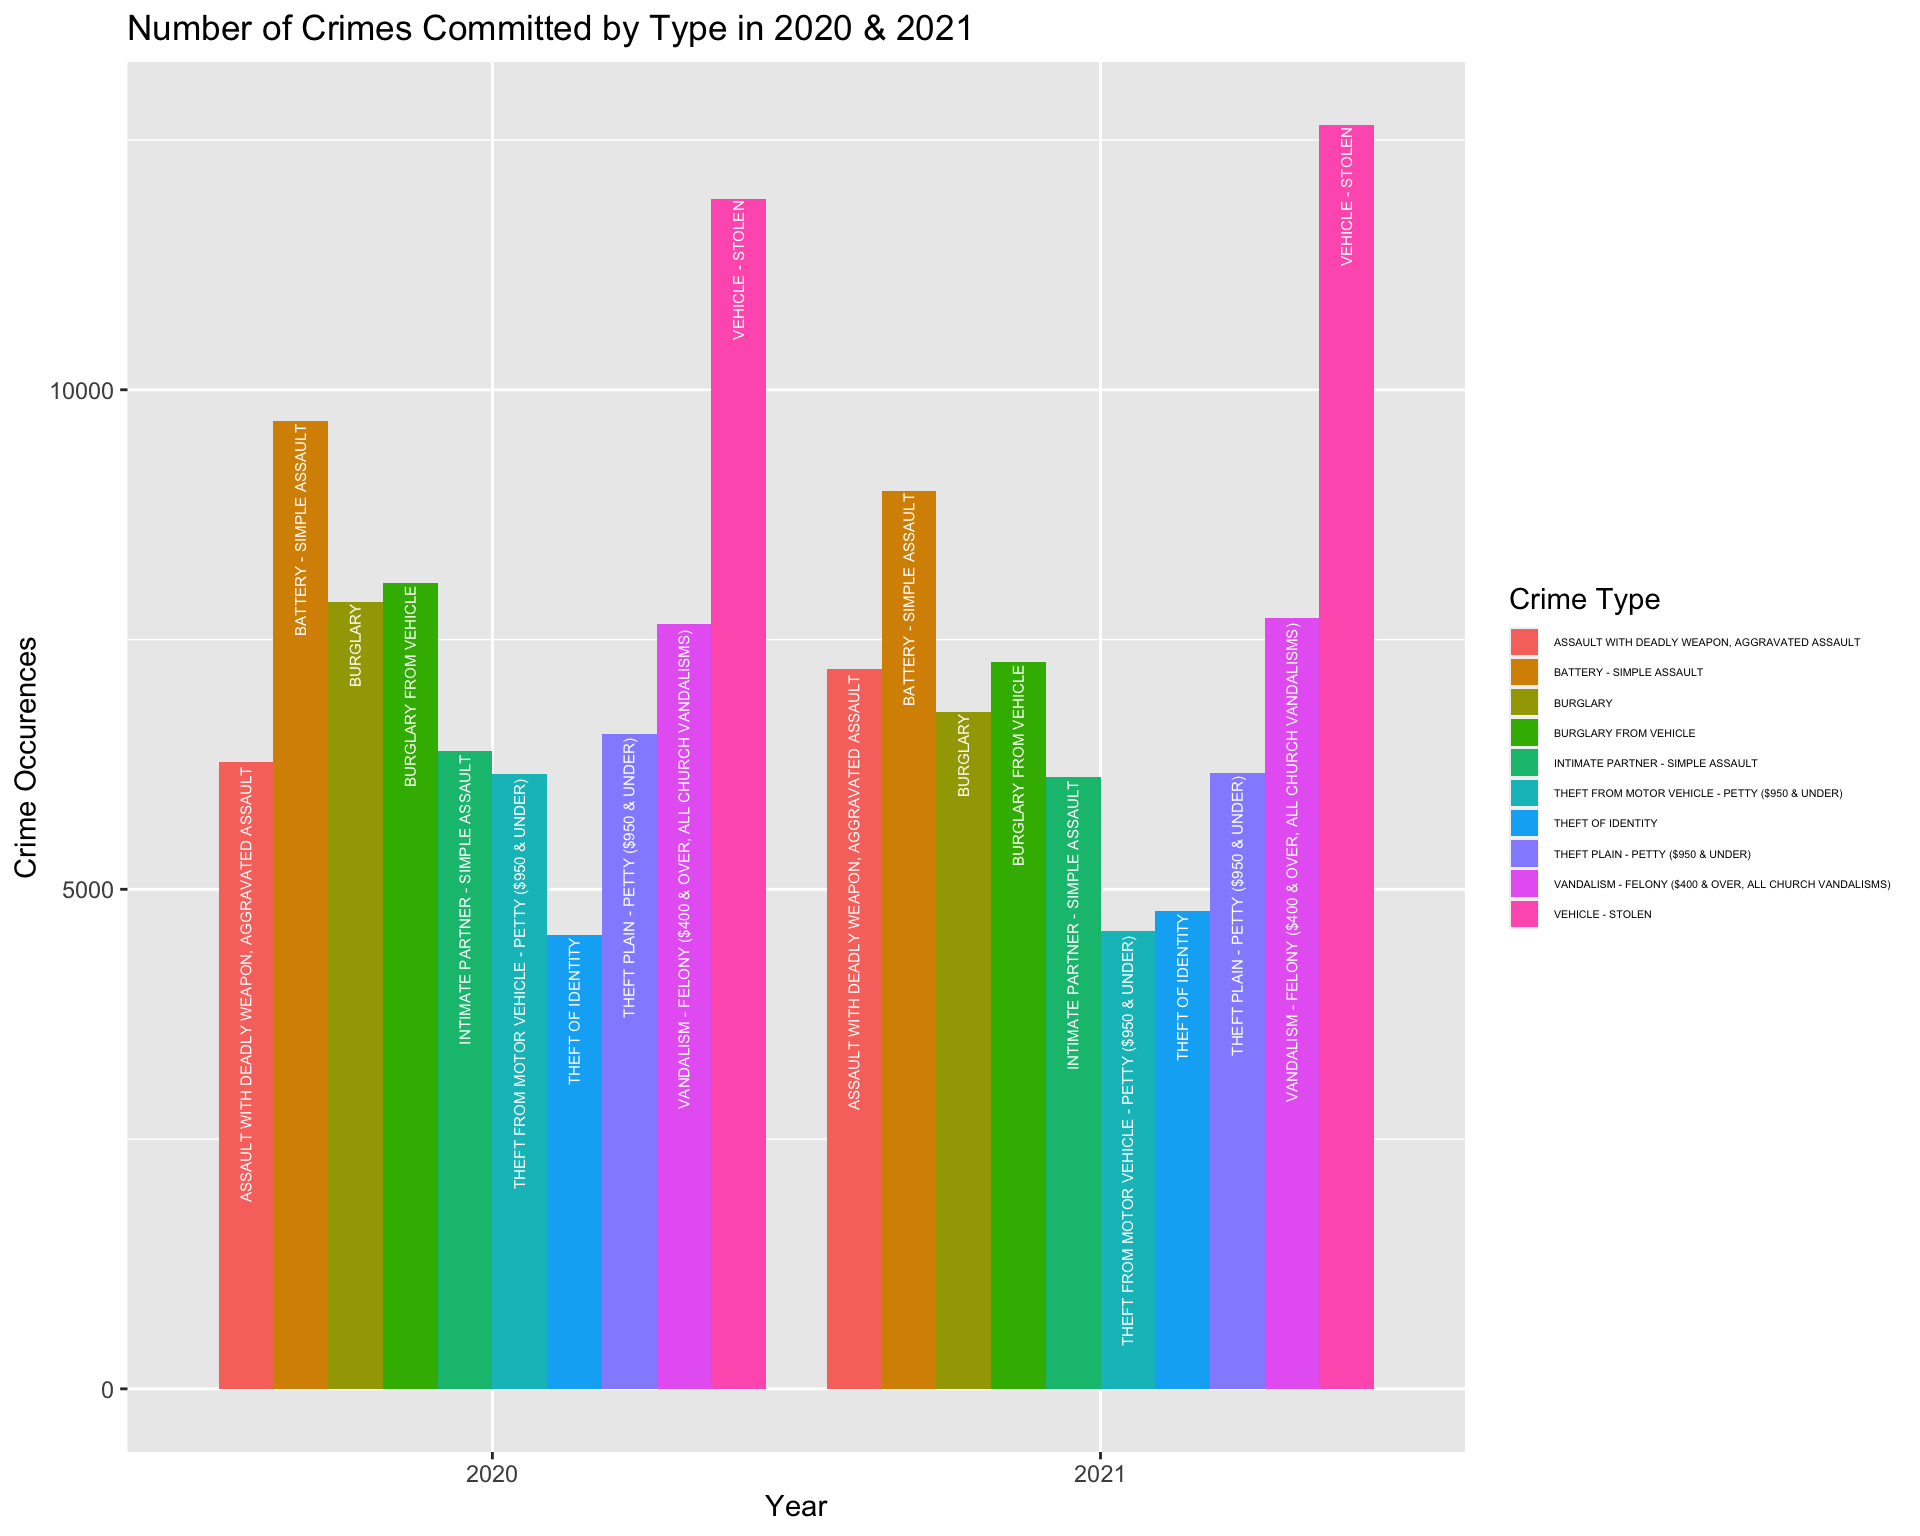
\includegraphics{StatMdlDecisionMaking_files/figure-latex/unnamed-chunk-4-1.pdf}

\begin{Shaded}
\begin{Highlighting}[]
  \FunctionTok{ggplot}\NormalTok{(infmort, }\FunctionTok{aes}\NormalTok{(}\AttributeTok{x =}\NormalTok{ income, }\AttributeTok{y =}\NormalTok{ mortality, }\AttributeTok{color =}\NormalTok{ region))}\SpecialCharTok{+}
    \FunctionTok{geom\_point}\NormalTok{(}\AttributeTok{alpha =} \FloatTok{0.7}\NormalTok{)}
\end{Highlighting}
\end{Shaded}

\includegraphics{StatMdlDecisionMaking_files/figure-latex/unnamed-chunk-4-2.pdf}

\begin{Shaded}
\begin{Highlighting}[]
  \CommentTok{\#Assumptions}
    \CommentTok{\#Assumptions}
    \CommentTok{\#1.Independent of residuals = Assumed in design of experiment. }
    \CommentTok{\#2.Linearity = Not linear.}
      \FunctionTok{par}\NormalTok{(}\AttributeTok{mfrow=}\FunctionTok{c}\NormalTok{(}\DecValTok{2}\NormalTok{,}\DecValTok{2}\NormalTok{))}
      \FunctionTok{plot}\NormalTok{(Reg)}
\end{Highlighting}
\end{Shaded}

\includegraphics{StatMdlDecisionMaking_files/figure-latex/unnamed-chunk-4-3.pdf}

\begin{Shaded}
\begin{Highlighting}[]
      \FunctionTok{crPlots}\NormalTok{(Reg) }\CommentTok{\#Residuals vs Fitted plot looks not straight.}
    \CommentTok{\#3 Homoscedasticity/ constant variability of resifduals = Not homoscedastic.}
      \FunctionTok{par}\NormalTok{(}\AttributeTok{mfrow=}\FunctionTok{c}\NormalTok{(}\DecValTok{2}\NormalTok{,}\DecValTok{2}\NormalTok{))}
\end{Highlighting}
\end{Shaded}

\includegraphics{StatMdlDecisionMaking_files/figure-latex/unnamed-chunk-4-4.pdf}

\begin{Shaded}
\begin{Highlighting}[]
      \FunctionTok{plot}\NormalTok{(Reg)}\CommentTok{\#Scale{-}Location plot is not straight.}
\end{Highlighting}
\end{Shaded}

\includegraphics{StatMdlDecisionMaking_files/figure-latex/unnamed-chunk-4-5.pdf}

\begin{Shaded}
\begin{Highlighting}[]
    \CommentTok{\#4 Normality of Residuals = Residuals are not normal. Skewed to the right \& kurtotic.}
      \CommentTok{\#See plot(Reg)\textquotesingle{}s Normal Q{-}Q plot OR the following: }
\NormalTok{      infmort.data }\OtherTok{\textless{}{-}} \FunctionTok{augment}\NormalTok{(Reg)}\CommentTok{\# get the residuals}
      \FunctionTok{ggplot}\NormalTok{(infmort.data, }\FunctionTok{aes}\NormalTok{(}\AttributeTok{sample =}\NormalTok{ .resid)) }\SpecialCharTok{+}
\FunctionTok{geom\_qq}\NormalTok{() }\SpecialCharTok{+}
\FunctionTok{stat\_qq\_line}\NormalTok{(}\AttributeTok{color =} \StringTok{"green"}\NormalTok{) }\CommentTok{\# The outliers are way off the line}
\end{Highlighting}
\end{Shaded}

\includegraphics{StatMdlDecisionMaking_files/figure-latex/unnamed-chunk-4-6.pdf}

\begin{Shaded}
\begin{Highlighting}[]
     \FunctionTok{ggplot}\NormalTok{(infmort.data, }\FunctionTok{aes}\NormalTok{(}\AttributeTok{x =}\NormalTok{ .resid)) }\SpecialCharTok{+}
\FunctionTok{geom\_histogram}\NormalTok{(}\AttributeTok{bins =} \DecValTok{25}\NormalTok{)}\CommentTok{\# Now this shows it isn\textquotesingle{}t normal. Right skewed \& kurtotic}
\end{Highlighting}
\end{Shaded}

\includegraphics{StatMdlDecisionMaking_files/figure-latex/unnamed-chunk-4-7.pdf}

\begin{Shaded}
\begin{Highlighting}[]
\NormalTok{     (}\FunctionTok{length}\NormalTok{(}\FunctionTok{boxplot}\NormalTok{(infmort}\SpecialCharTok{$}\NormalTok{mortality, }\AttributeTok{plot=}\NormalTok{F)}\SpecialCharTok{$}\NormalTok{out)}\SpecialCharTok{/}\DecValTok{101}\NormalTok{)}\SpecialCharTok{*}\DecValTok{100} \CommentTok{\#I could remove outliers here, but I\textquotesingle{}ve decided against it since 3\% of the data are outliers. That seems like a lot to cut out.}
\end{Highlighting}
\end{Shaded}

\begin{verbatim}
## [1] 2.970297
\end{verbatim}

\begin{Shaded}
\begin{Highlighting}[]
\CommentTok{\#Dummy variable  }
\NormalTok{infmortDum }\OtherTok{\textless{}{-}} \FunctionTok{mutate}\NormalTok{(infmort, }\AttributeTok{region.dum =} \FunctionTok{factor}\NormalTok{(region))}
\NormalTok{Reg\_Dum }\OtherTok{\textless{}{-}} \FunctionTok{lm}\NormalTok{(mortality}\SpecialCharTok{\textasciitilde{}}\NormalTok{region.dum, infmortDum)}
\FunctionTok{summary}\NormalTok{(Reg\_Dum)}
\end{Highlighting}
\end{Shaded}

\begin{verbatim}
## 
## Call:
## lm(formula = mortality ~ region.dum, data = infmortDum)
## 
## Residuals:
##    Min     1Q Median     3Q    Max 
## -87.29 -37.52  -5.76  16.91 553.83 
## 
## Coefficients:
##                    Estimate Std. Error t value Pr(>|t|)    
## (Intercept)          142.29      13.64  10.431  < 2e-16 ***
## region.dumAmericas   -87.17      21.76  -4.005 0.000122 ***
## region.dumAsia       -46.12      20.50  -2.249 0.026755 *  
## region.dumEurope    -123.04      23.19  -5.306 7.07e-07 ***
## ---
## Signif. codes:  0 '***' 0.001 '**' 0.01 '*' 0.05 '.' 0.1 ' ' 1
## 
## Residual standard error: 79.54 on 97 degrees of freedom
## Multiple R-squared:  0.2556, Adjusted R-squared:  0.2326 
## F-statistic:  11.1 on 3 and 97 DF,  p-value: 2.494e-06
\end{verbatim}

\begin{Shaded}
\begin{Highlighting}[]
\CommentTok{\#2 Answer}
\NormalTok{interaction }\OtherTok{\textless{}{-}} \FunctionTok{lm}\NormalTok{(mortality }\SpecialCharTok{\textasciitilde{}}\NormalTok{ region.dum }\SpecialCharTok{*}\NormalTok{ income, }\AttributeTok{data =}\NormalTok{ infmortDum)}
\FunctionTok{summary}\NormalTok{(interaction)}
\end{Highlighting}
\end{Shaded}

\begin{verbatim}
## 
## Call:
## lm(formula = mortality ~ region.dum * income, data = infmortDum)
## 
## Residuals:
##     Min      1Q  Median      3Q     Max 
## -101.04  -31.36   -2.58   16.25  559.77 
## 
## Coefficients:
##                            Estimate Std. Error t value Pr(>|t|)    
## (Intercept)               130.91725   15.55534   8.416 4.55e-13 ***
## region.dumAmericas        -66.30647   26.15577  -2.535   0.0129 *  
## region.dumAsia            -30.28530   24.14769  -1.254   0.2129    
## region.dumEurope          -96.26275   47.63292  -2.021   0.0462 *  
## income                      0.04163    0.02702   1.541   0.1268    
## region.dumAmericas:income  -0.05133    0.02982  -1.721   0.0886 .  
## region.dumAsia:income      -0.04842    0.03121  -1.552   0.1242    
## region.dumEurope:income    -0.04669    0.03018  -1.547   0.1253    
## ---
## Signif. codes:  0 '***' 0.001 '**' 0.01 '*' 0.05 '.' 0.1 ' ' 1
## 
## Residual standard error: 79.83 on 93 degrees of freedom
## Multiple R-squared:  0.2811, Adjusted R-squared:  0.227 
## F-statistic: 5.194 on 7 and 93 DF,  p-value: 5.055e-05
\end{verbatim}

\begin{Shaded}
\begin{Highlighting}[]
\CommentTok{\#Tried log to make it more normal, but it didn\textquotesingle{}t do much}
\NormalTok{interaction.log }\OtherTok{\textless{}{-}} \FunctionTok{lm}\NormalTok{(}\FunctionTok{log}\NormalTok{(mortality) }\SpecialCharTok{\textasciitilde{}}\NormalTok{ region.dum }\SpecialCharTok{*}\NormalTok{ income, }\AttributeTok{data =}\NormalTok{ infmortDum)}
\NormalTok{infmort.data2 }\OtherTok{\textless{}{-}} \FunctionTok{augment}\NormalTok{(interaction.log)}
\FunctionTok{ggplot}\NormalTok{(infmort.data2, }\FunctionTok{aes}\NormalTok{(}\AttributeTok{sample =}\NormalTok{ .std.resid)) }\SpecialCharTok{+}
\FunctionTok{geom\_qq}\NormalTok{() }\SpecialCharTok{+}
\FunctionTok{stat\_qq\_line}\NormalTok{(}\AttributeTok{color =} \StringTok{"green"}\NormalTok{) }
\end{Highlighting}
\end{Shaded}

\includegraphics{StatMdlDecisionMaking_files/figure-latex/unnamed-chunk-4-8.pdf}

\end{document}
